\begin{frame}{Far-field Bistatic RCS calculation}{Reference cases}

The same geometry is analized with different orientations of the longitudinal axis:

\vbs

\begin{columns}

\column{0.4\textwidth}
\includegraphics[width=\linewidth]
{results/3D/20/300/\meshCCC{01}{1}{075}/geometry.pdf}

\column{0.55\textwidth}

\begin{itemize}

\item Normal incidence
\item Dashed black line:
\item Blue line: $S'$
\item Red line: $S$
\item Different values of permittivity between PEC and $S'$: $\varepsilon_r$
\item $f=300$\,MHz ($\lambda=1$\,m, cylinder radius is $5\lambda$).

\end{itemize}

\end{columns}

\end{frame}

\begin{frame}{TM polarization, $\varepsilon_r=1$ (reference case)}


\begin{columns}
\column{0.23\textwidth}

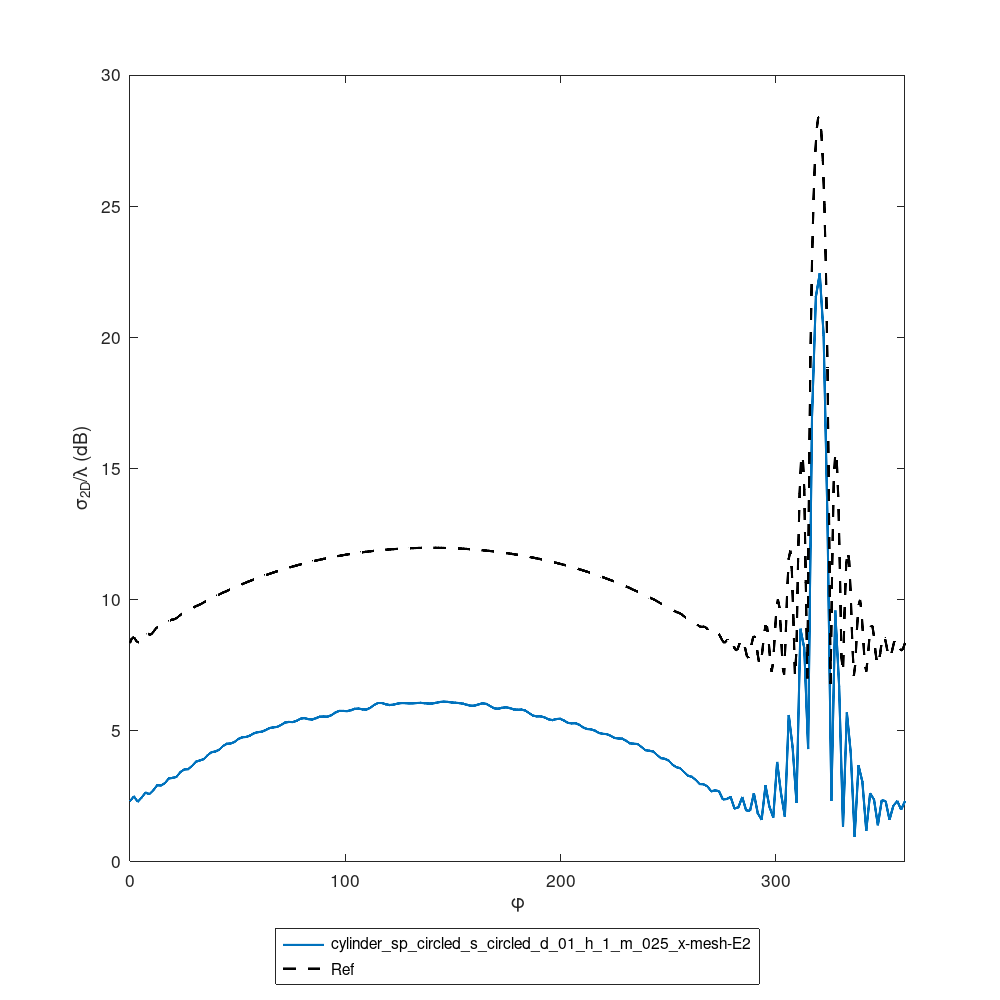
\includegraphics[width=\linewidth]{results/FF/cylD_01_H_1_M_025_X/iiee.png}

\column{0.23\textwidth}

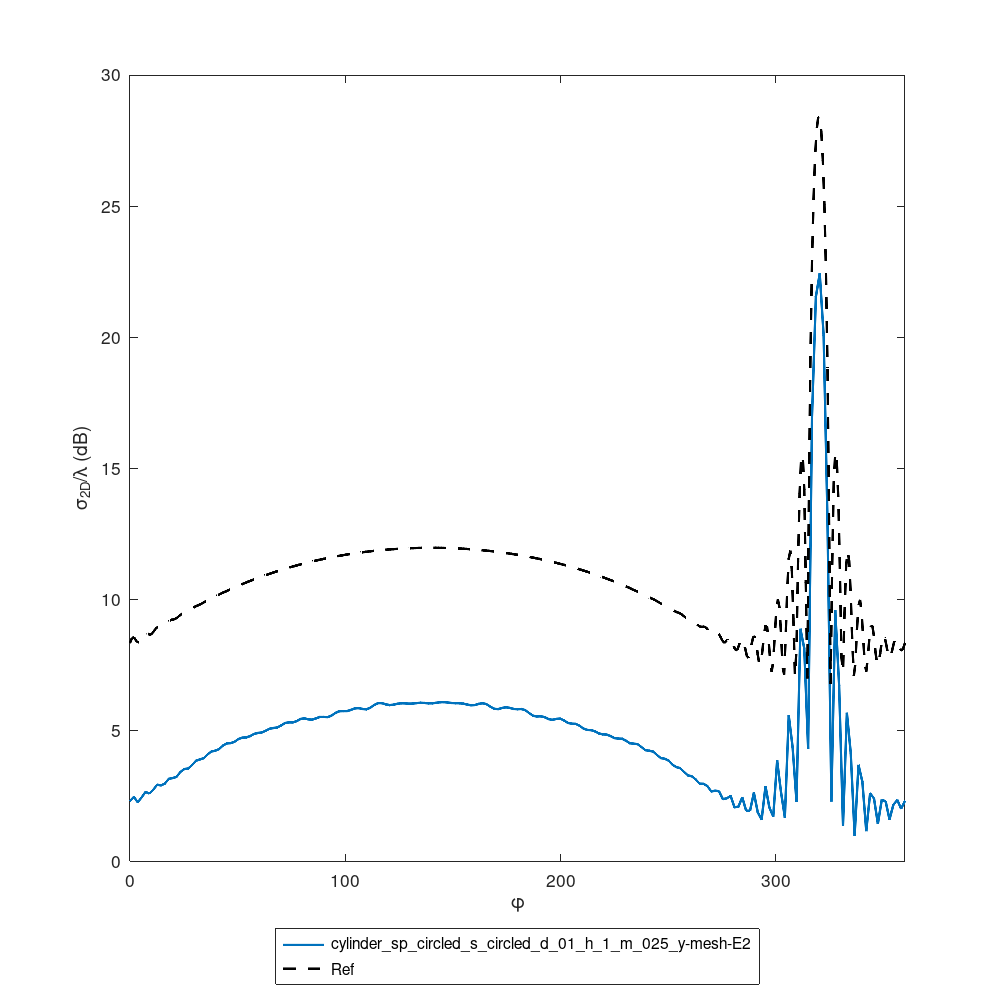
\includegraphics[width=\linewidth]{results/FF/cylD_01_H_1_M_025_Y/iiee.png}

\column{0.23\textwidth}

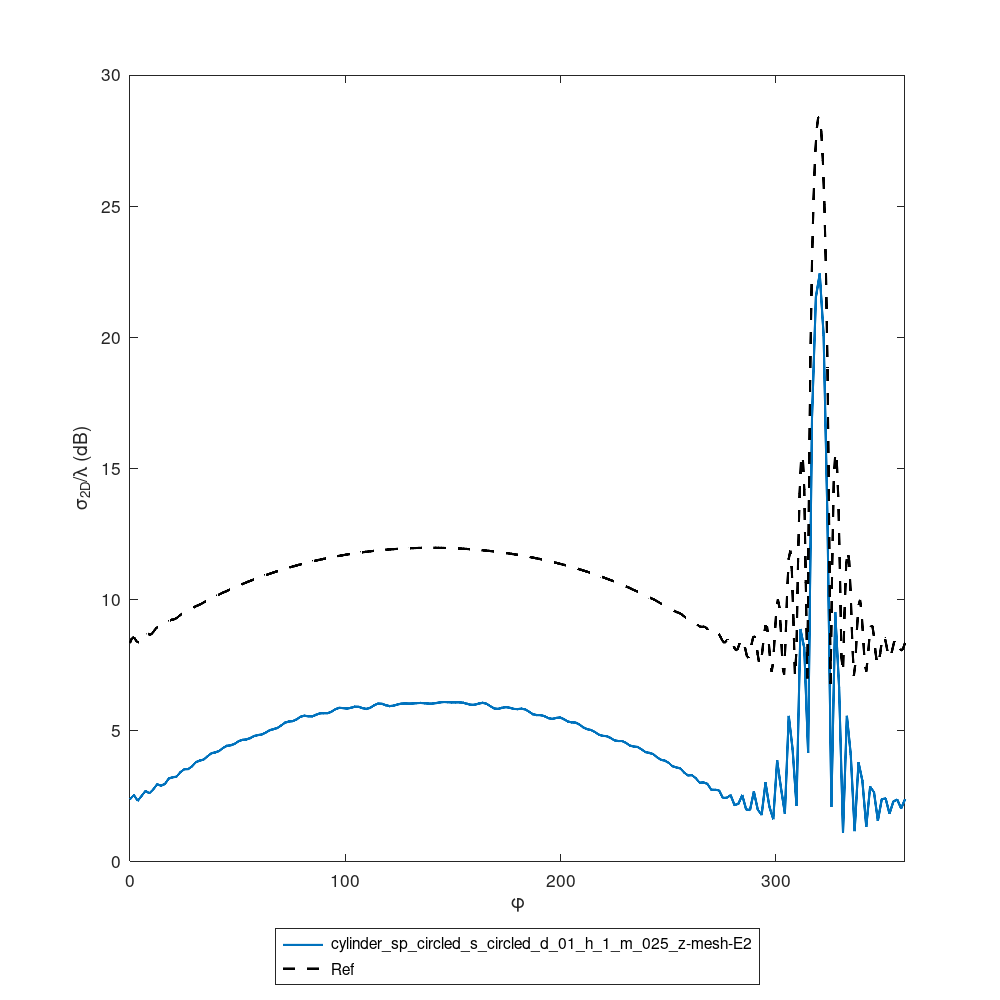
\includegraphics[width=\linewidth]{results/FF/cylD_01_H_1_M_025_Z/iiee.png}

\column{0.23\textwidth}

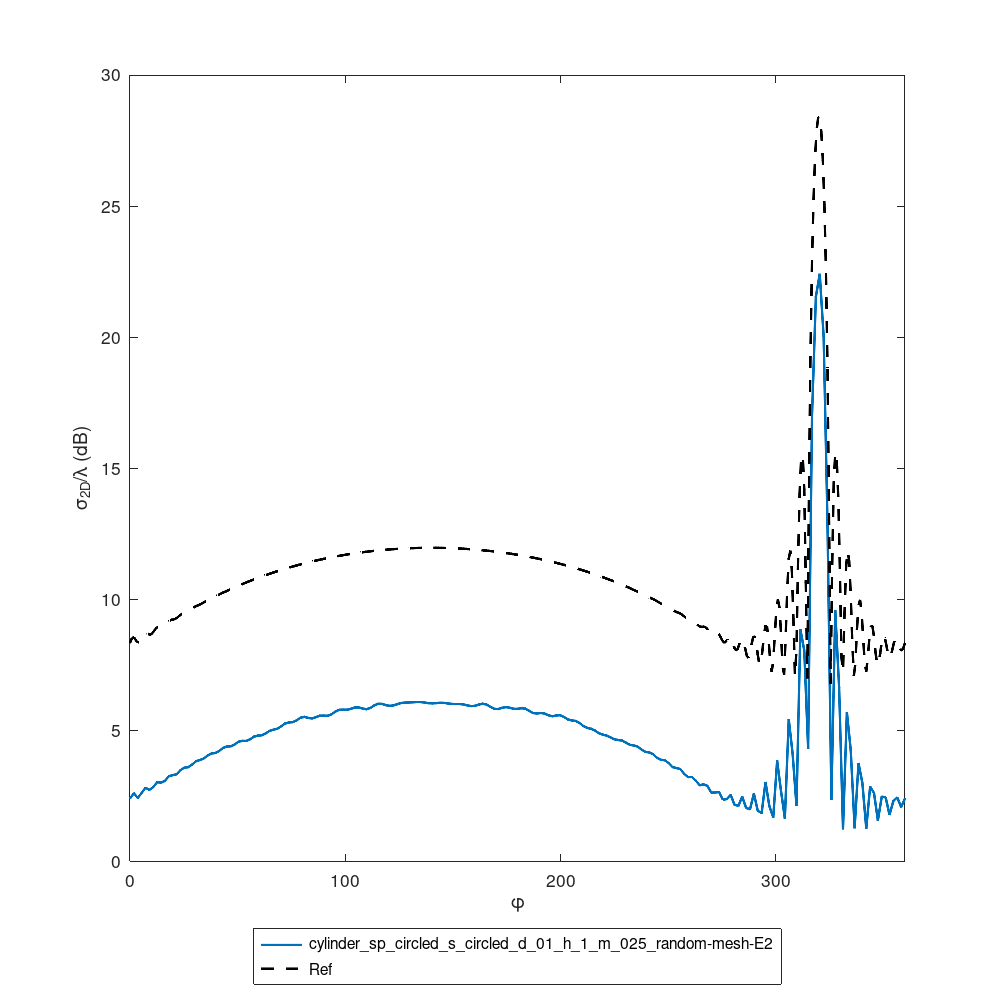
\includegraphics[width=\linewidth]{results/FF/cylD_01_H_1_M_025_RANDOM/iiee.png}

\end{columns}

\vbs

Analytical curves and FEM curves agree except for a constant factor.
\alert{DEBO ACTUALIZAR ESTO QUE YA ESTA SUPERADO}

Normalized bistatic-RCS:

\vbss

\begin{columns}
\column{0.23\textwidth}

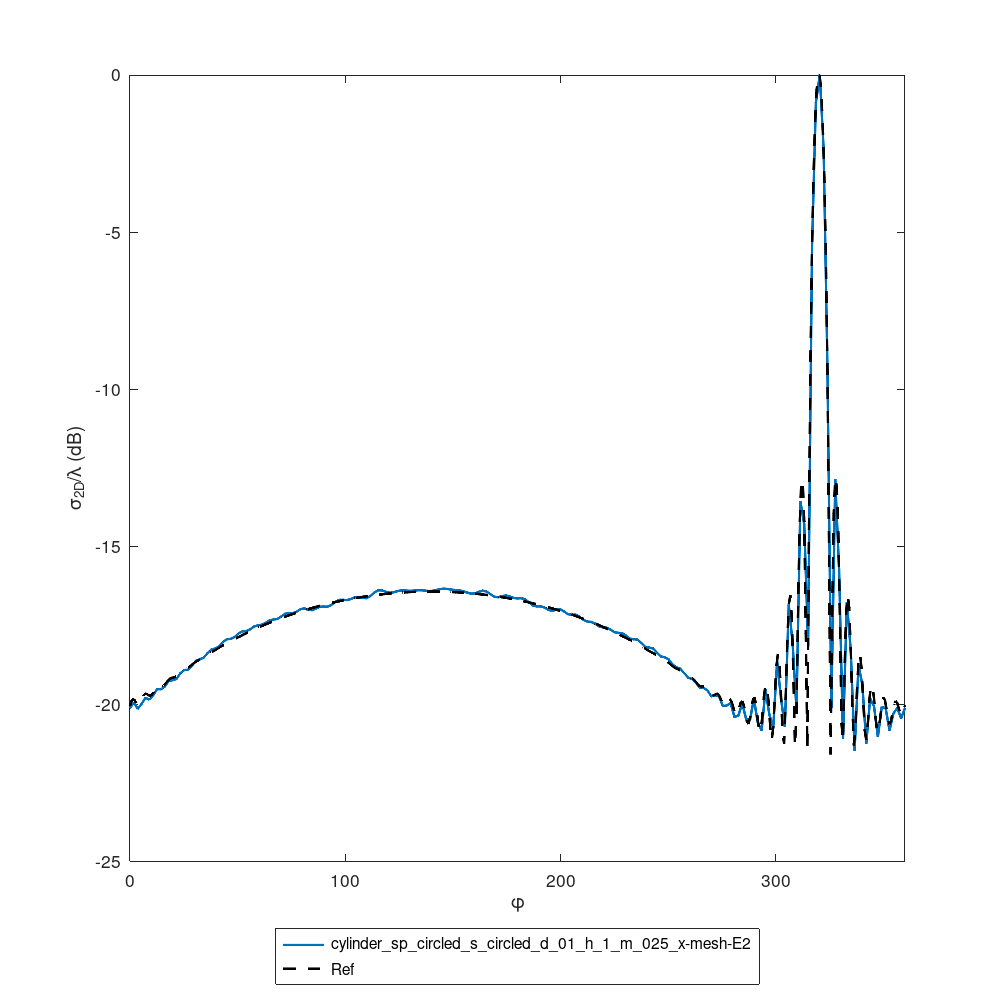
\includegraphics[width=\linewidth]{results/FF/cylD_01_H_1_M_025_X/iiee_norm.png}

\column{0.23\textwidth}

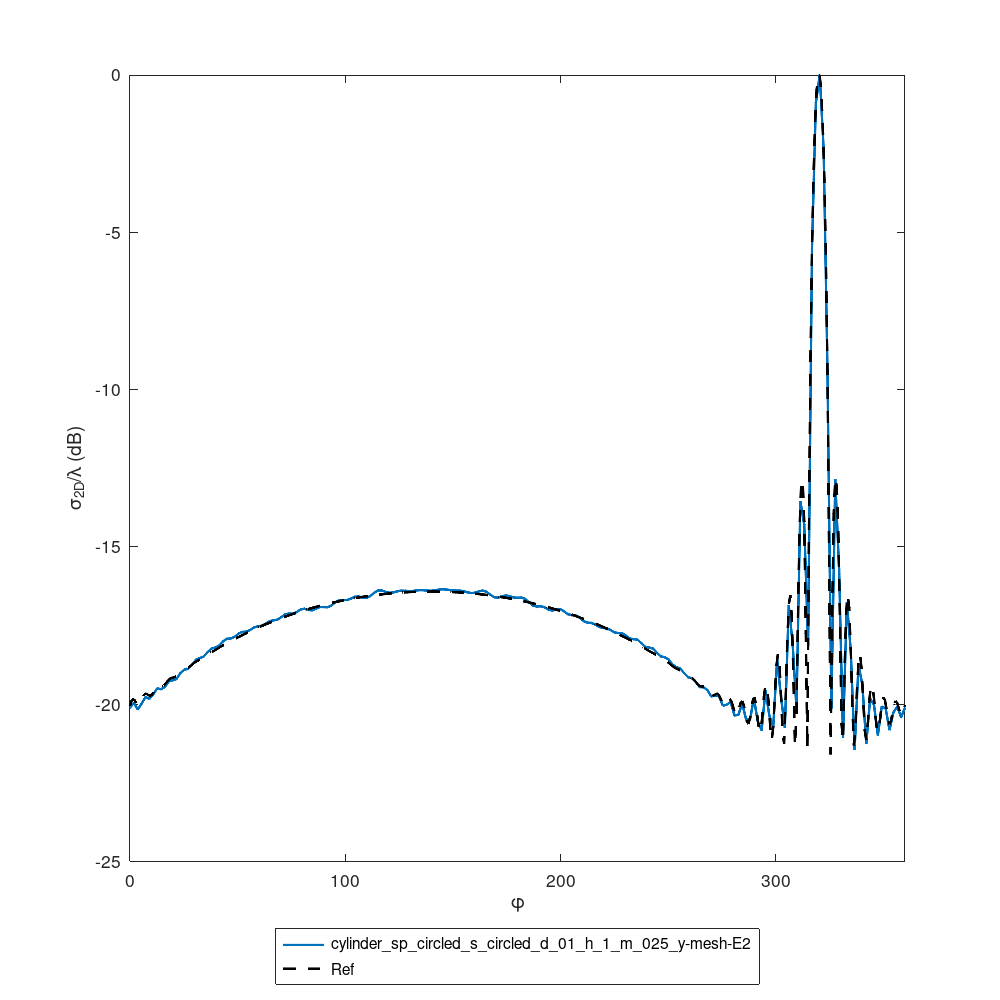
\includegraphics[width=\linewidth]{results/FF/cylD_01_H_1_M_025_Y/iiee_norm.png}

\column{0.23\textwidth}

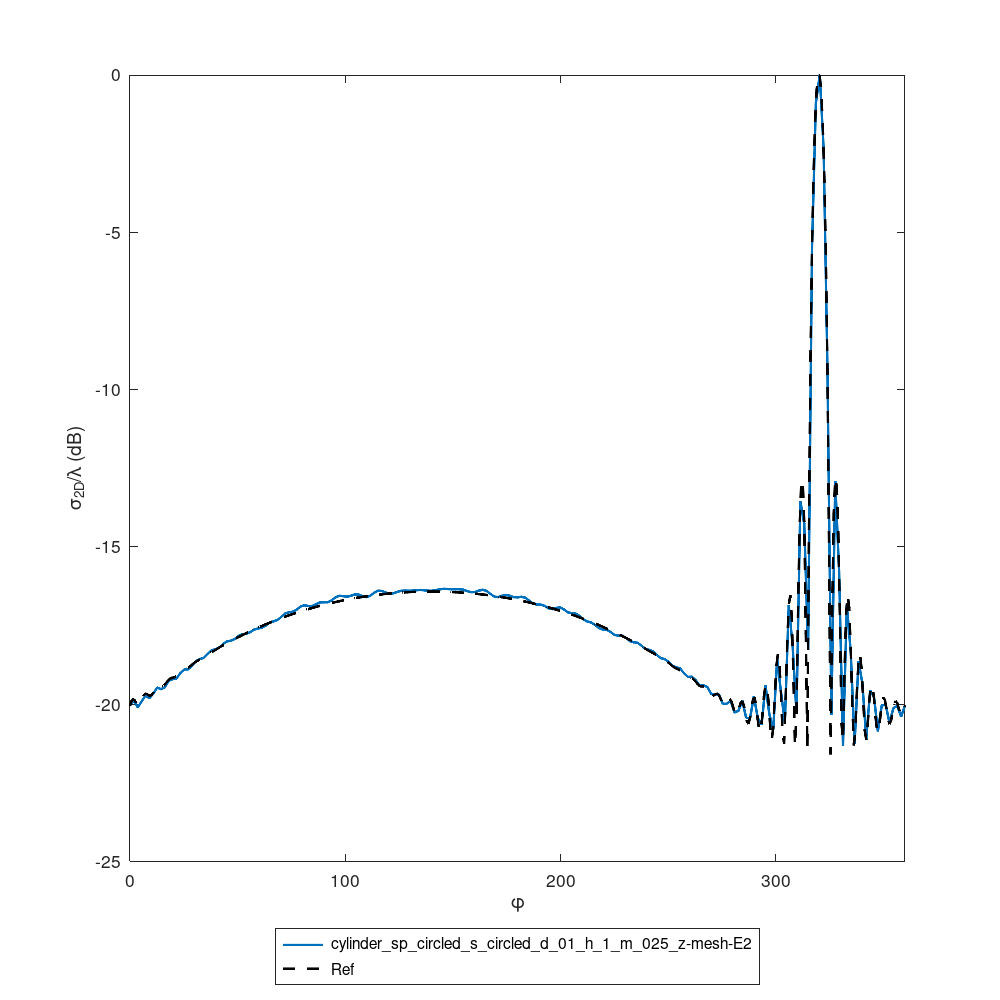
\includegraphics[width=\linewidth]{results/FF/cylD_01_H_1_M_025_Z/iiee_norm.png}

\column{0.23\textwidth}

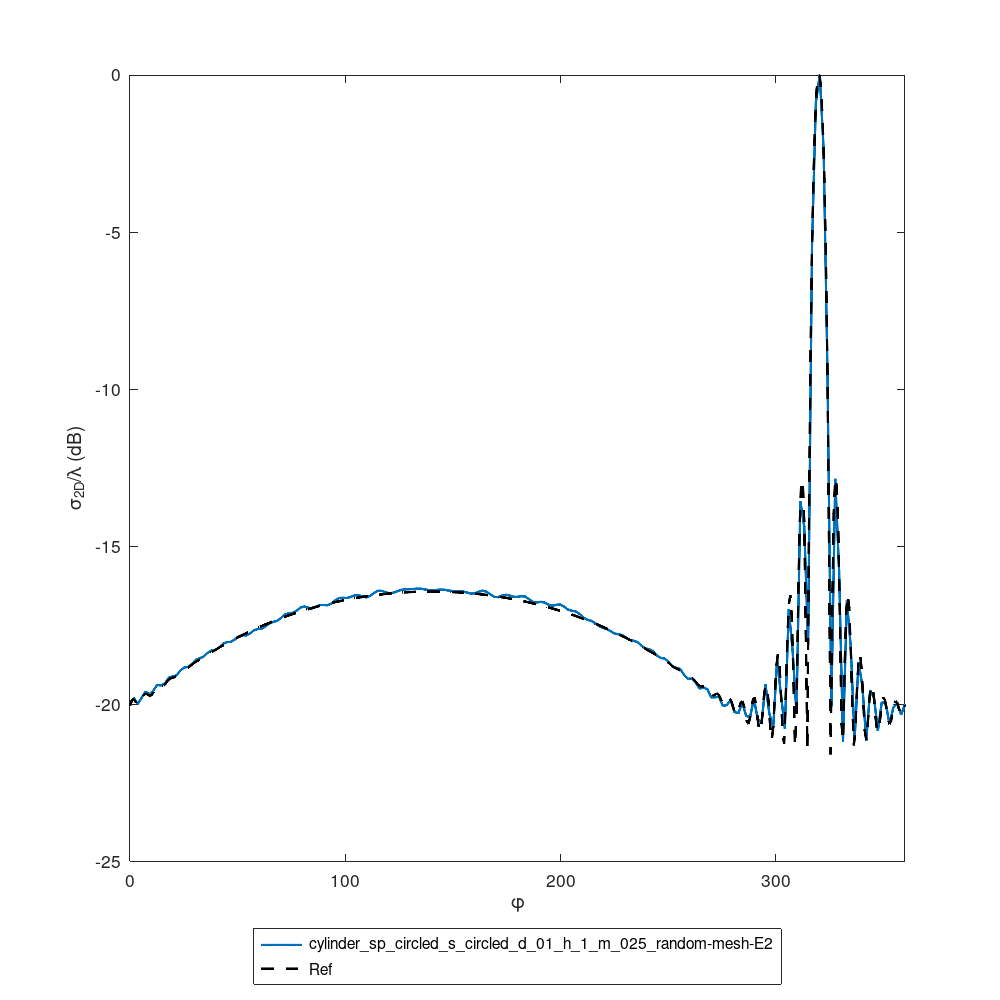
\includegraphics[width=\linewidth]{results/FF/cylD_01_H_1_M_025_RANDOM/iiee_norm.png}

\end{columns}


\end{frame}

%%%%%%%%%%%%%%%%%%%%%%%%%%%%%%%%%%%%%%%%

\begin{frame}{TE polarization, $\varepsilon_r=1$}

\begin{columns}
\column{0.23\textwidth}

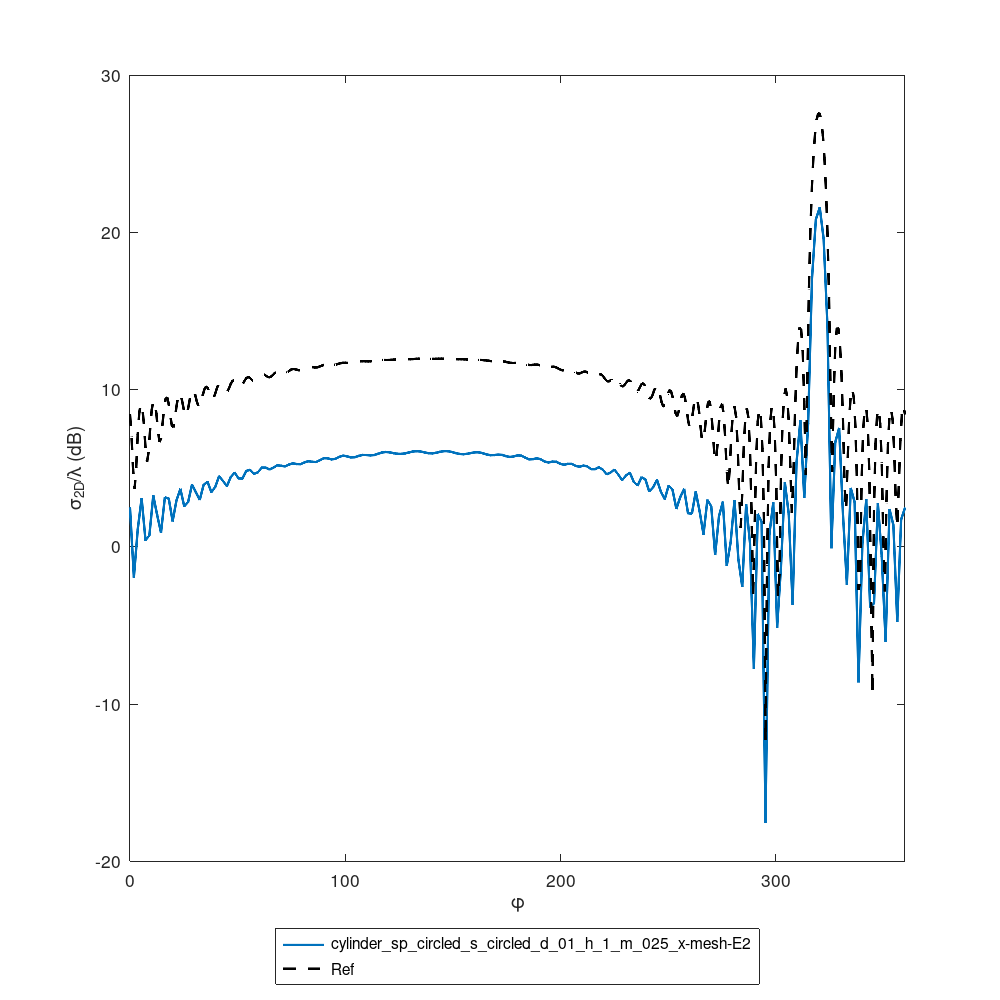
\includegraphics[width=\linewidth]{results/FF/cylD_01_H_1_M_025_X/epr1_TE.png}

\column{0.23\textwidth}

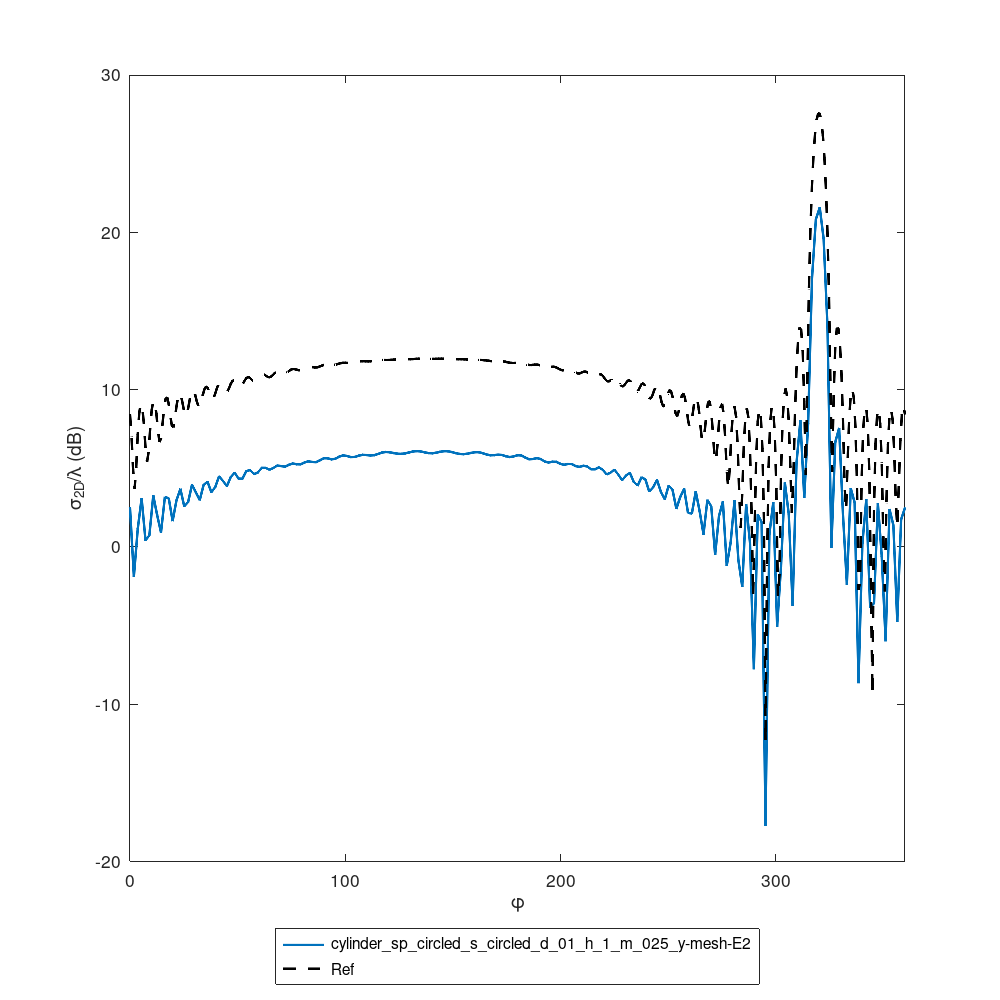
\includegraphics[width=\linewidth]{results/FF/cylD_01_H_1_M_025_Y/epr1_TE.png}

\column{0.23\textwidth}

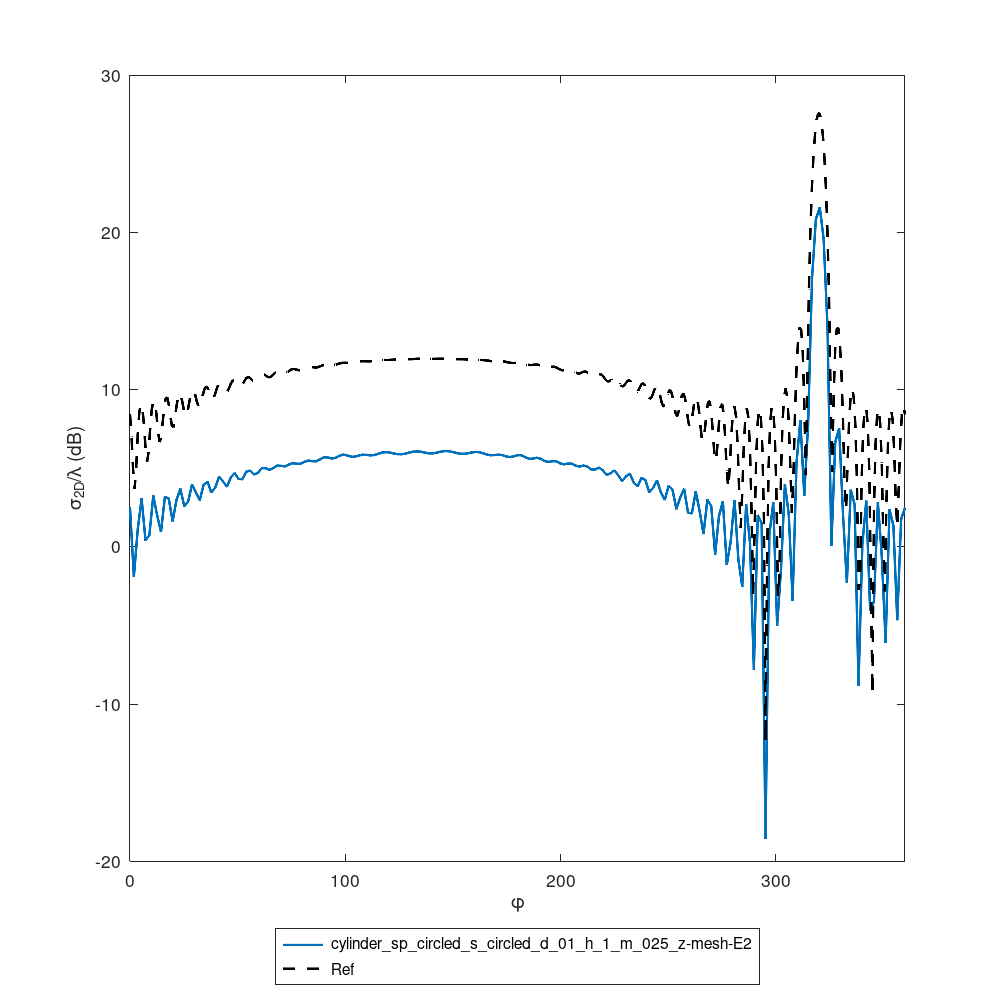
\includegraphics[width=\linewidth]{results/FF/cylD_01_H_1_M_025_Z/epr1_TE.png}

\column{0.23\textwidth}

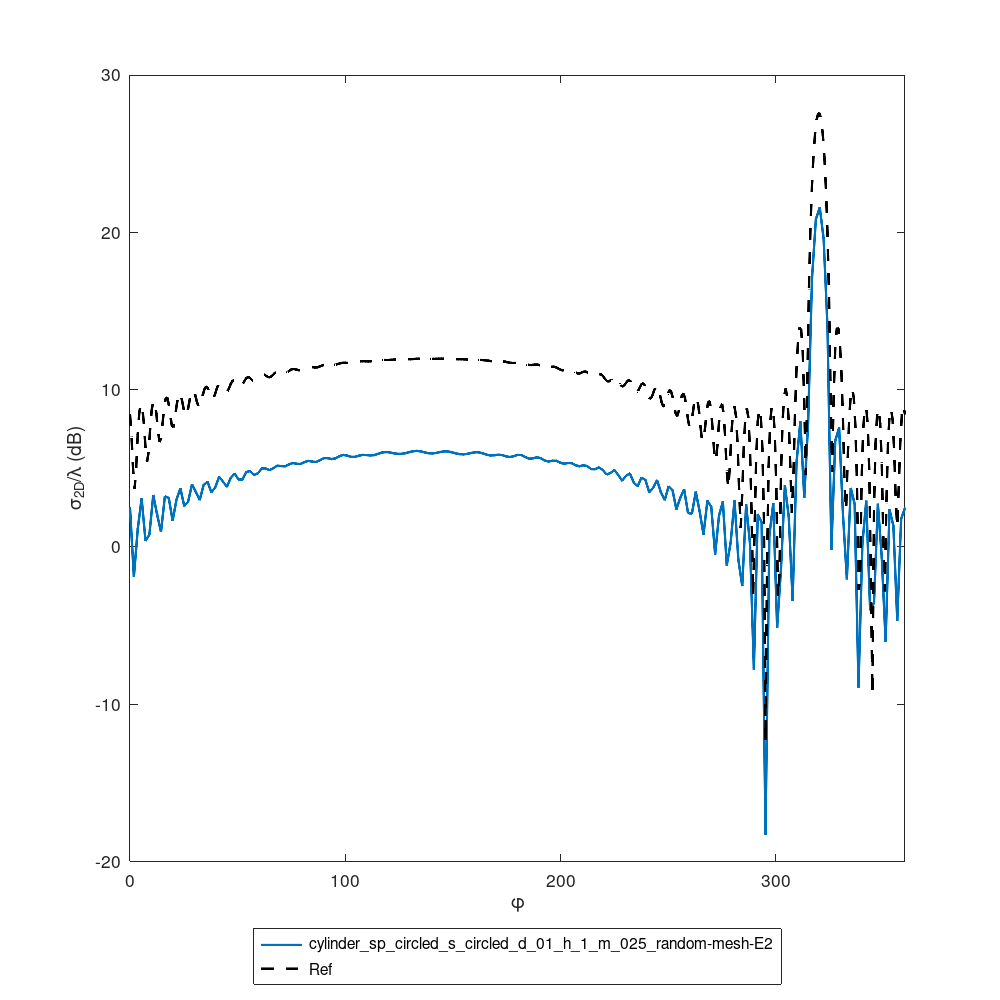
\includegraphics[width=\linewidth]{results/FF/cylD_01_H_1_M_025_RANDOM/epr1_TE.png}

\end{columns}

\vbs

Analytical curves and FEM curves agree except for a constant factor. 

Normalized bistatic-RCS:

\vbss

\begin{columns}
\column{0.23\textwidth}

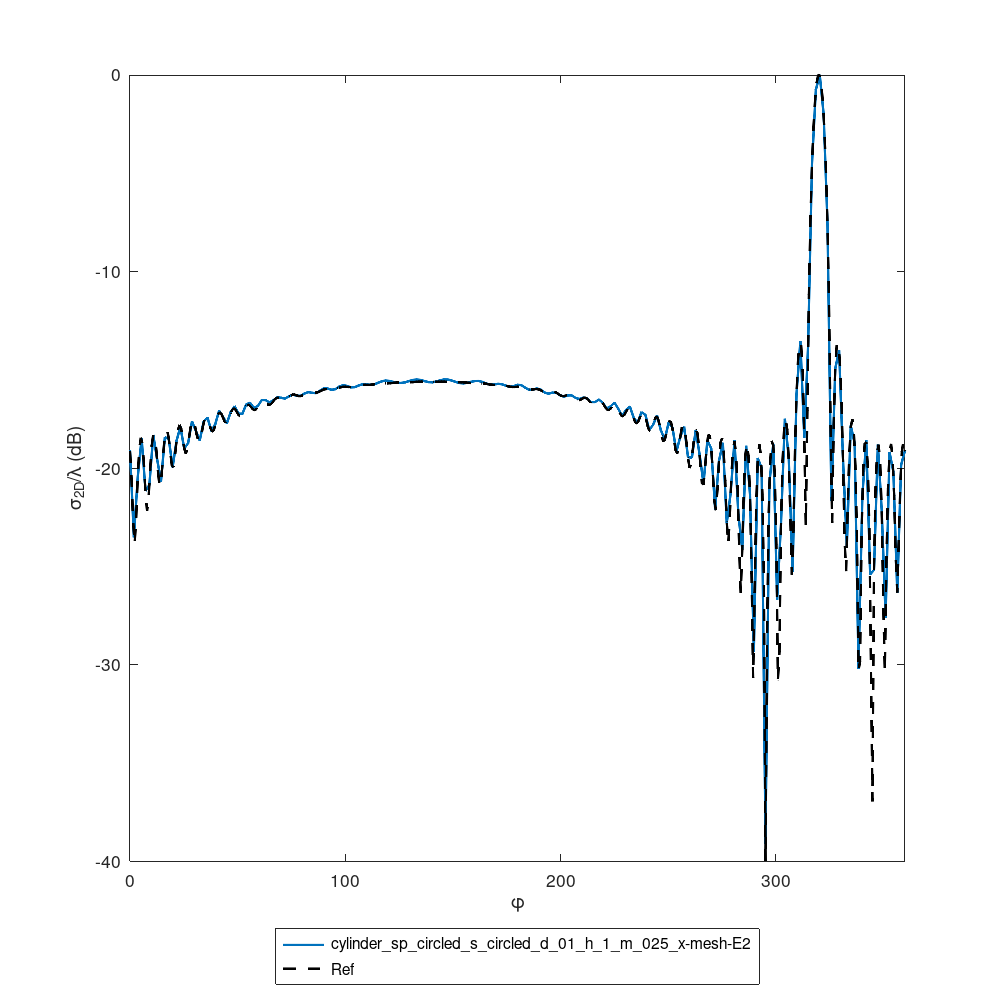
\includegraphics[width=\linewidth]{results/FF/cylD_01_H_1_M_025_X/epr1_TE_norm.png}

\column{0.23\textwidth}

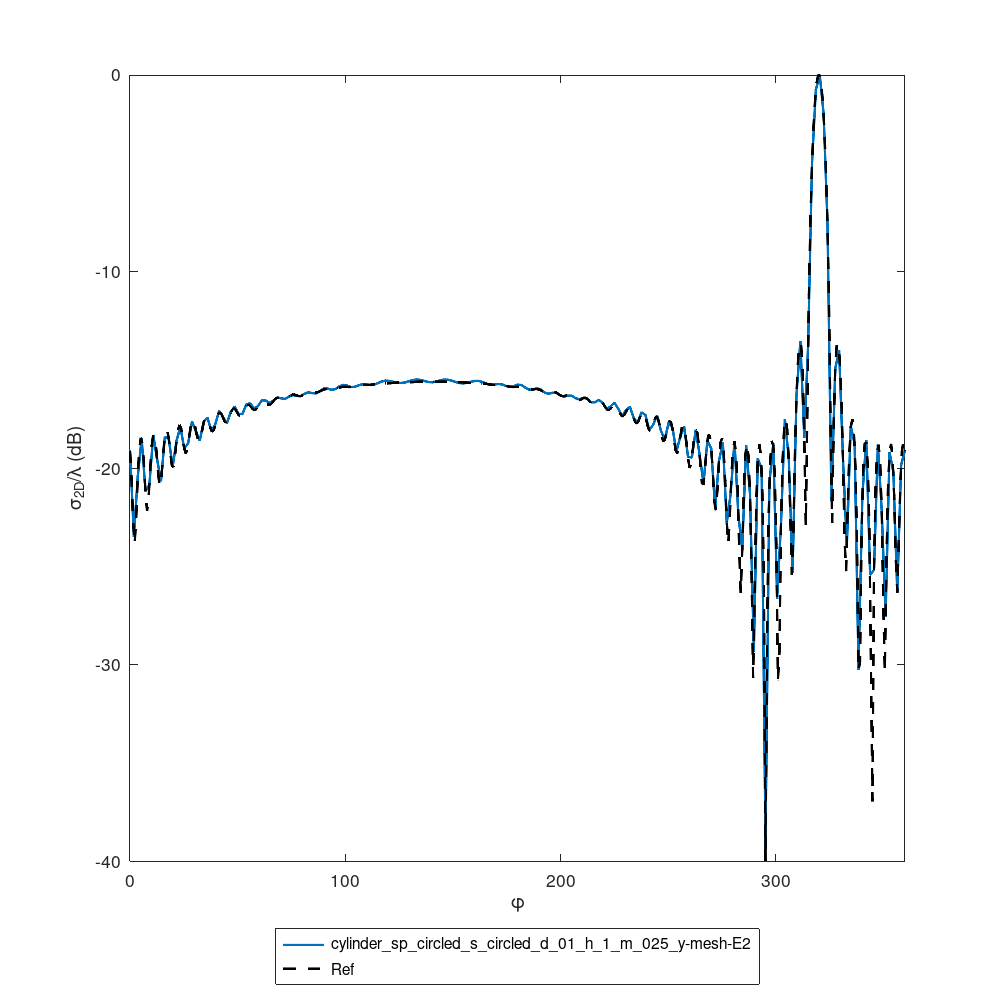
\includegraphics[width=\linewidth]{results/FF/cylD_01_H_1_M_025_Y/epr1_TE_norm.png}

\column{0.23\textwidth}

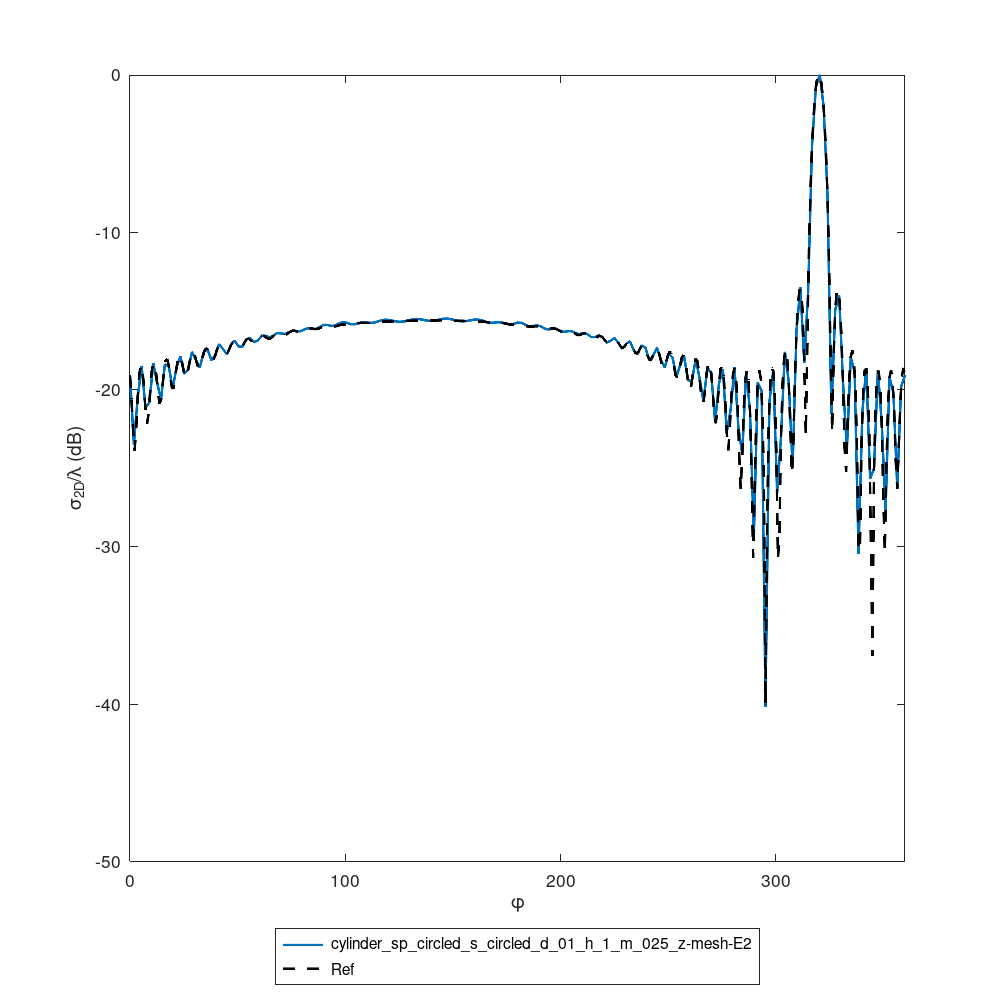
\includegraphics[width=\linewidth]{results/FF/cylD_01_H_1_M_025_Z/epr1_TE_norm.png}

\column{0.23\textwidth}

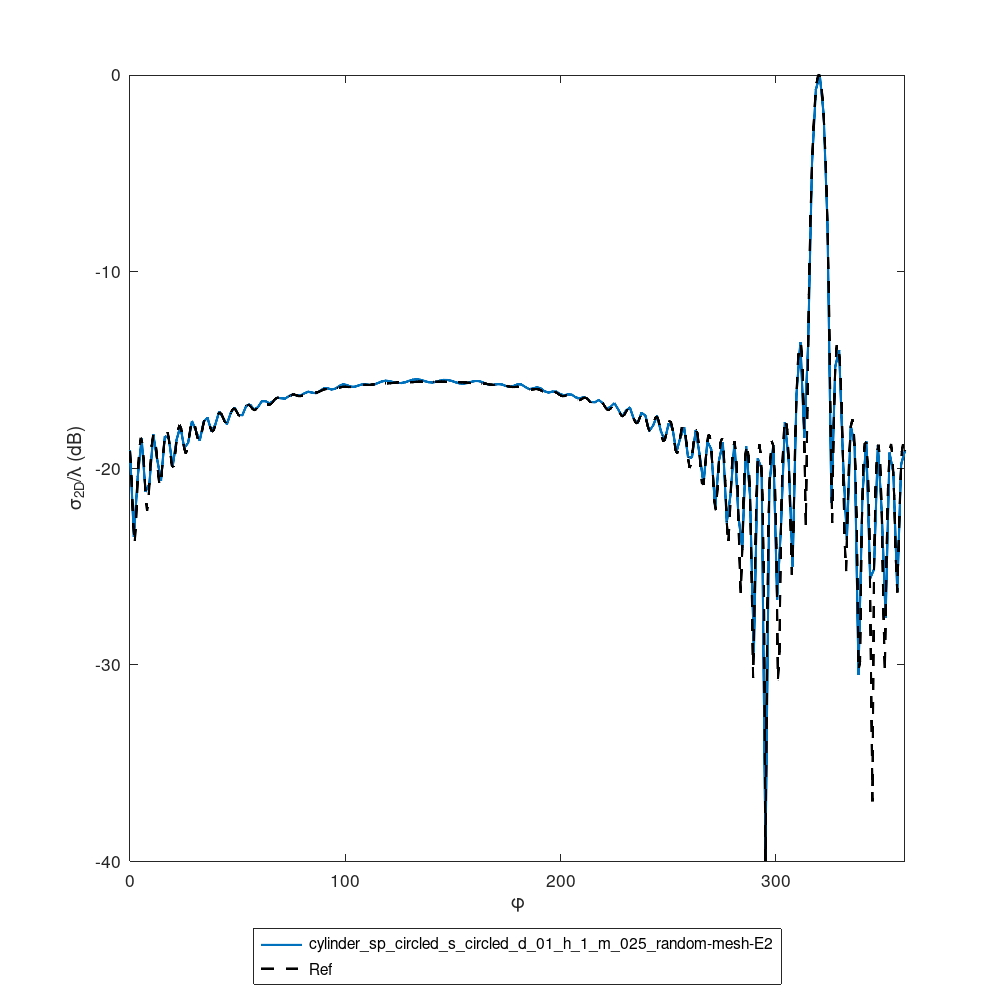
\includegraphics[width=\linewidth]{results/FF/cylD_01_H_1_M_025_RANDOM/epr1_TE_norm.png}

\end{columns}



\end{frame}

%%%%%%%%%%%%%%%%%%%%%%%%%%%%%%%%%%%%%%%%

\begin{frame}{TM polarization, $\varepsilon_r=8$}

\begin{columns}
\column{0.23\textwidth}

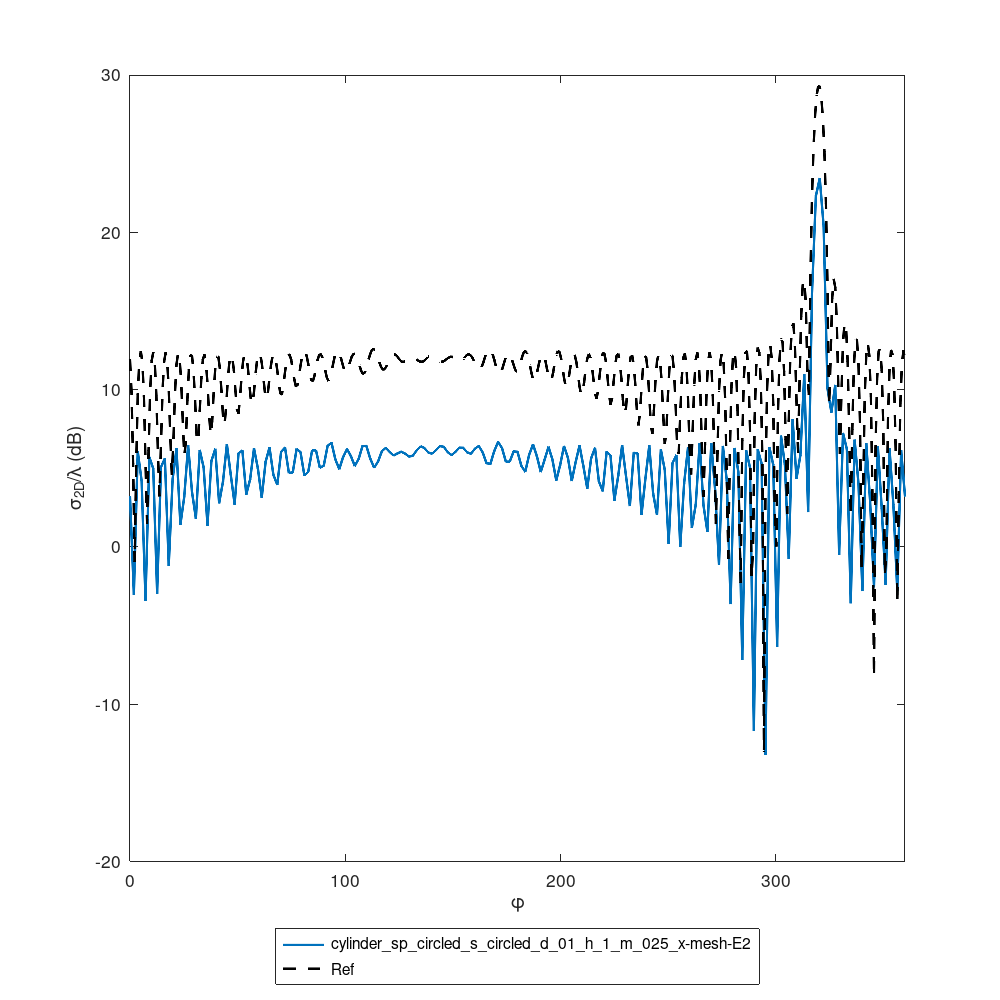
\includegraphics[width=\linewidth]{results/FF/cylD_01_H_1_M_025_X/epr8_TM.png}

\column{0.23\textwidth}

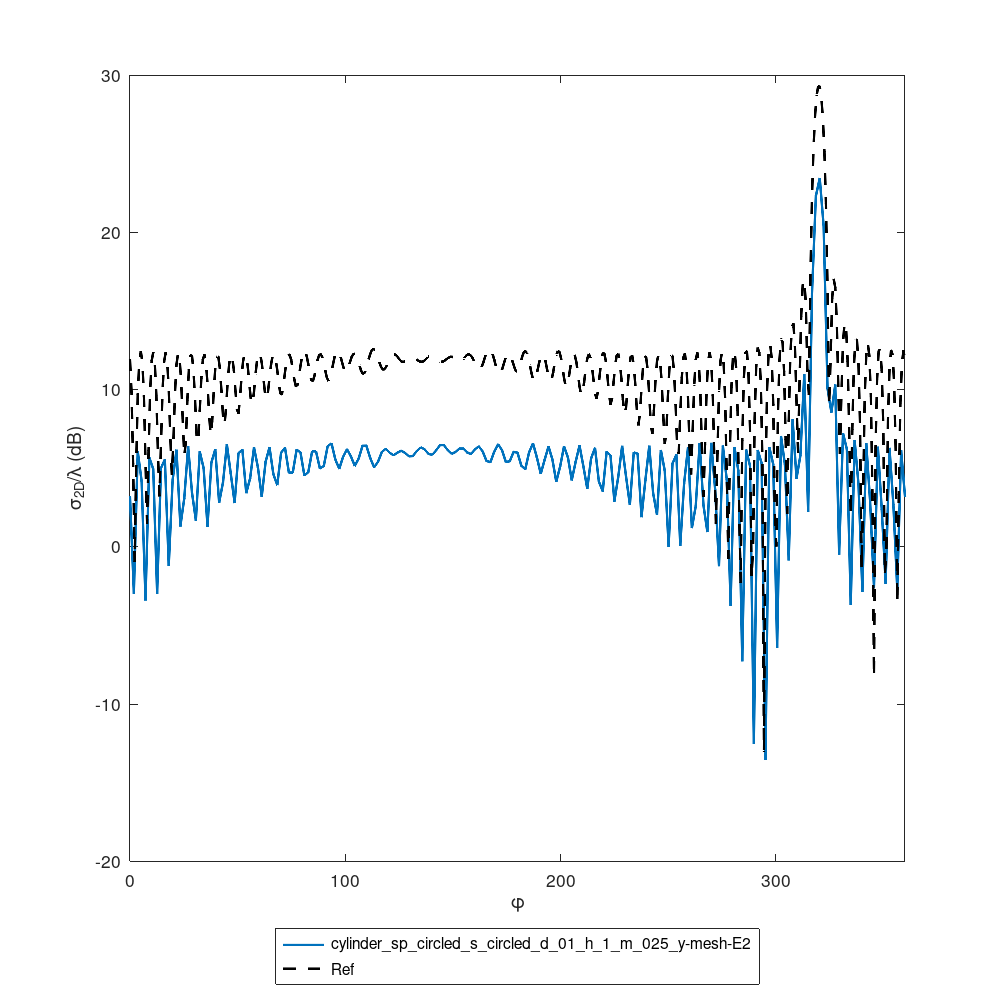
\includegraphics[width=\linewidth]{results/FF/cylD_01_H_1_M_025_Y/epr8_TM.png}

\column{0.23\textwidth}

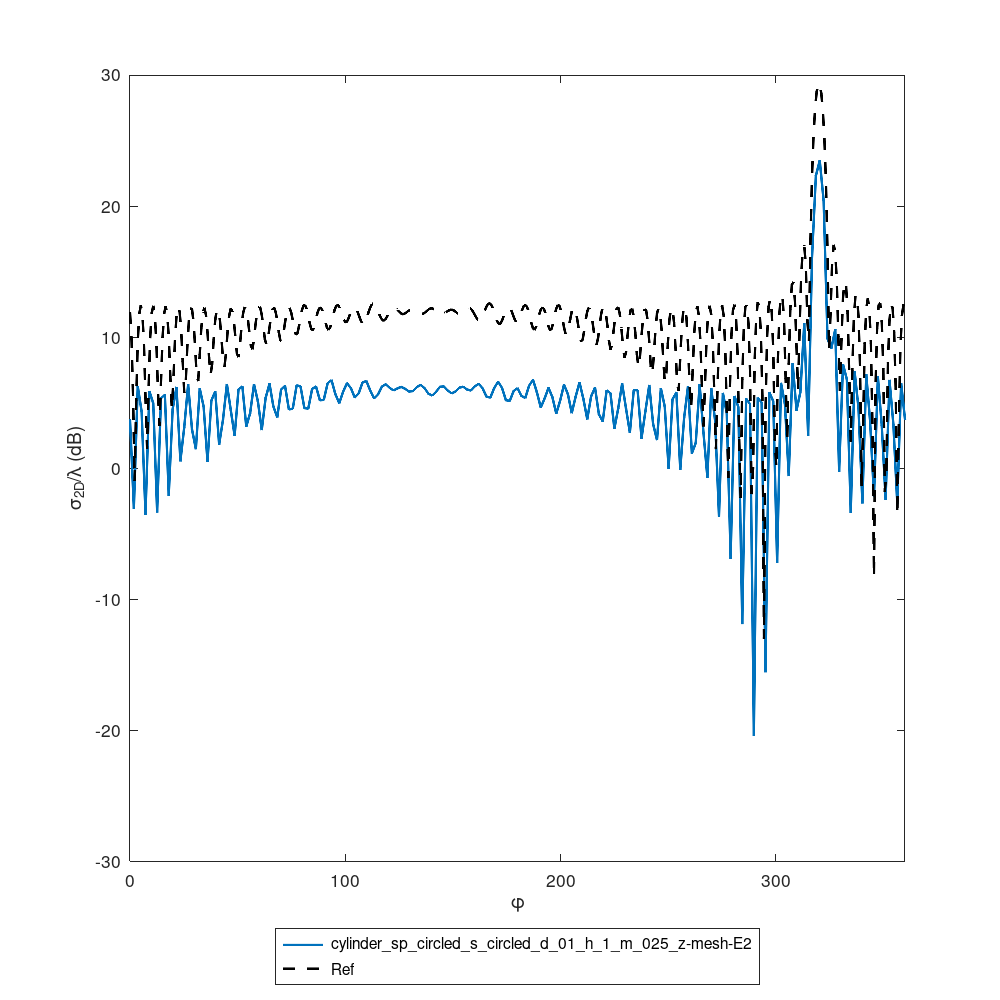
\includegraphics[width=\linewidth]{results/FF/cylD_01_H_1_M_025_Z/epr8_TM.png}

\column{0.23\textwidth}

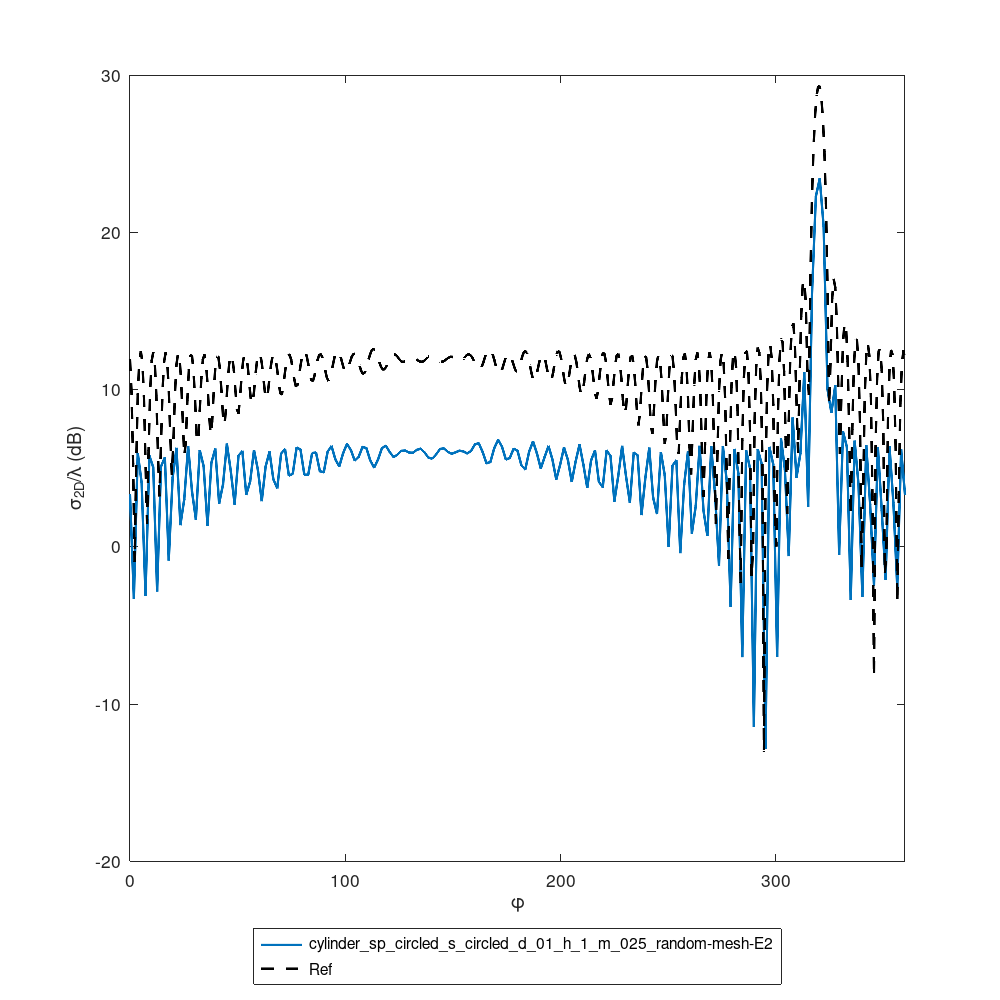
\includegraphics[width=\linewidth]{results/FF/cylD_01_H_1_M_025_RANDOM/epr8_TM.png}

\end{columns}

\vbs

Analytical curves and FEM curves agree (minor discrepancies) except for a constant factor. 

Normalized bistatic-RCS:

\vbss

\begin{columns}
\column{0.23\textwidth}

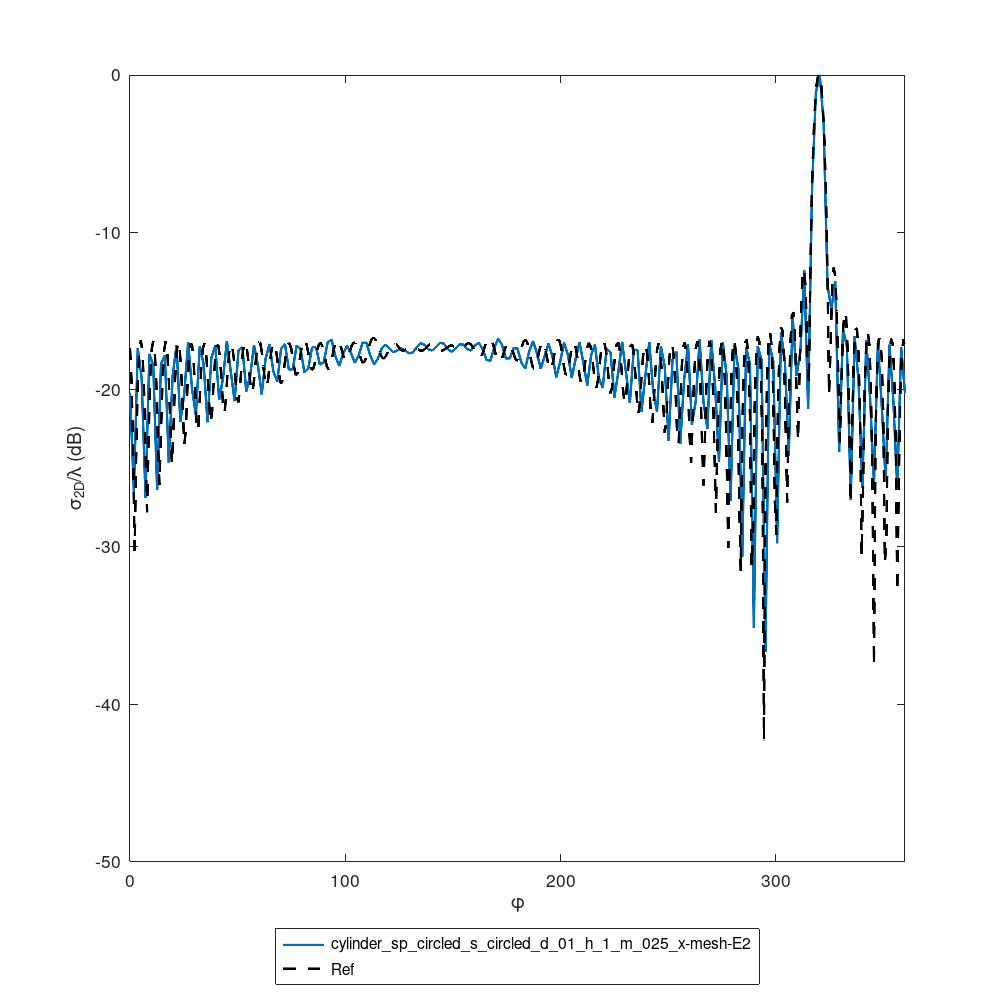
\includegraphics[width=\linewidth]{results/FF/cylD_01_H_1_M_025_X/epr8_TM_norm.png}

\column{0.23\textwidth}

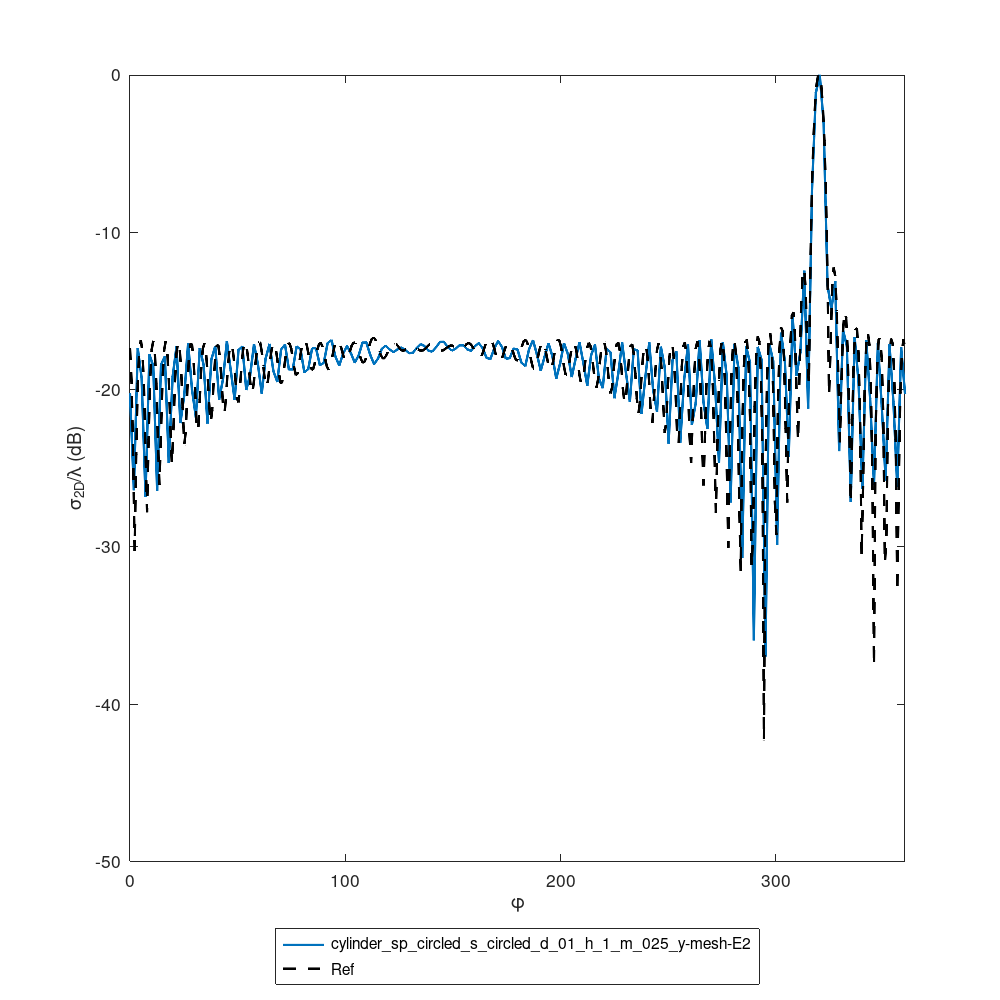
\includegraphics[width=\linewidth]{results/FF/cylD_01_H_1_M_025_Y/epr8_TM_norm.png}

\column{0.23\textwidth}

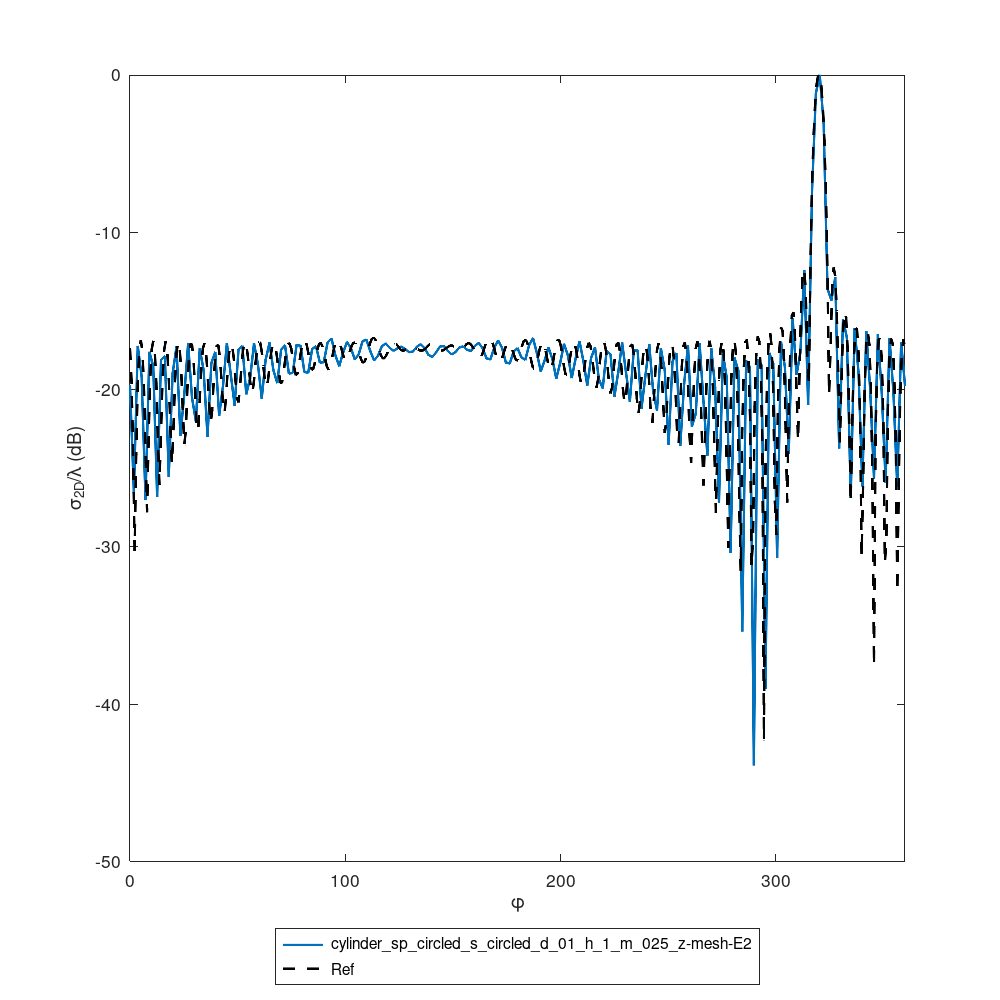
\includegraphics[width=\linewidth]{results/FF/cylD_01_H_1_M_025_Z/epr8_TM_norm.png}

\column{0.23\textwidth}

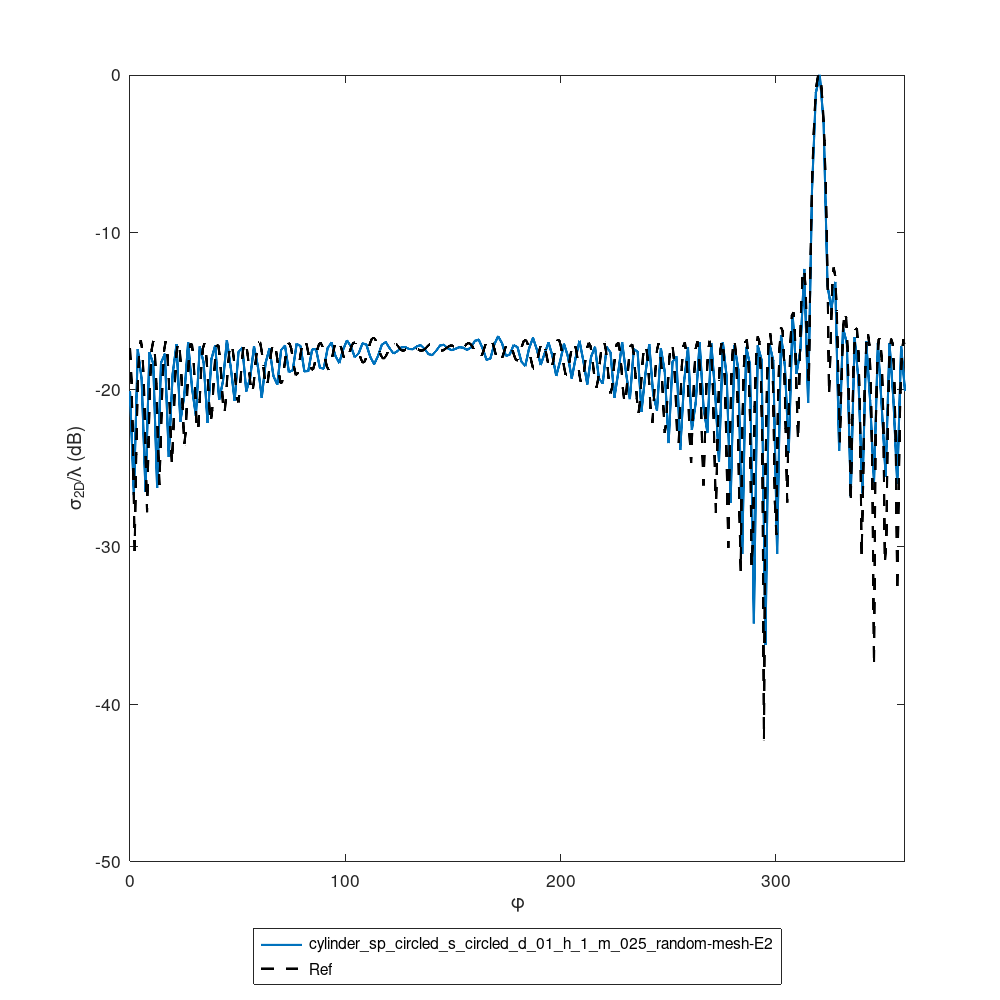
\includegraphics[width=\linewidth]{results/FF/cylD_01_H_1_M_025_RANDOM/epr8_TM_norm.png}

\end{columns}



\end{frame}


%%%%%%%%%%%%%%%%%%%%%%%%%%%%%%%%%%%%%%%%

\begin{frame}{TE polarization, $\varepsilon_r=2$}

\begin{columns}
\column{0.23\textwidth}

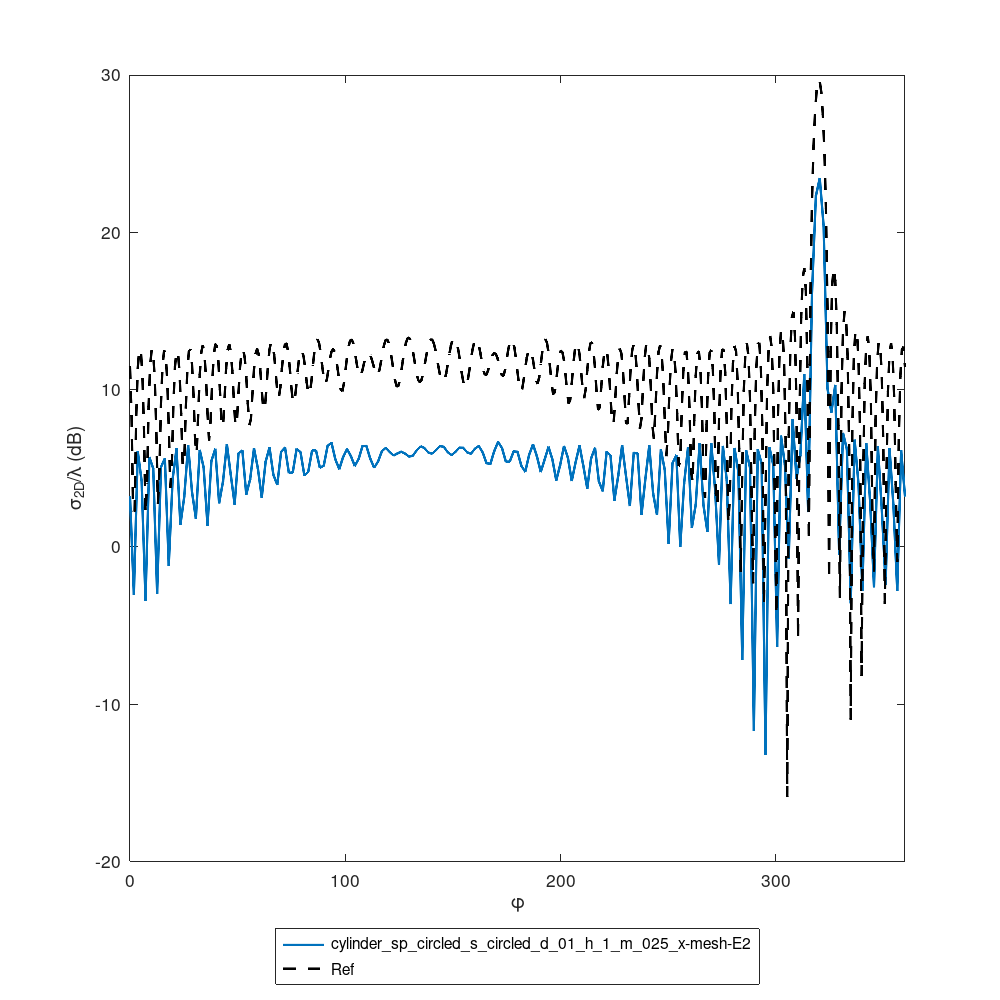
\includegraphics[width=\linewidth]{results/FF/cylD_01_H_1_M_025_X/epr2_TE.png}

\column{0.23\textwidth}

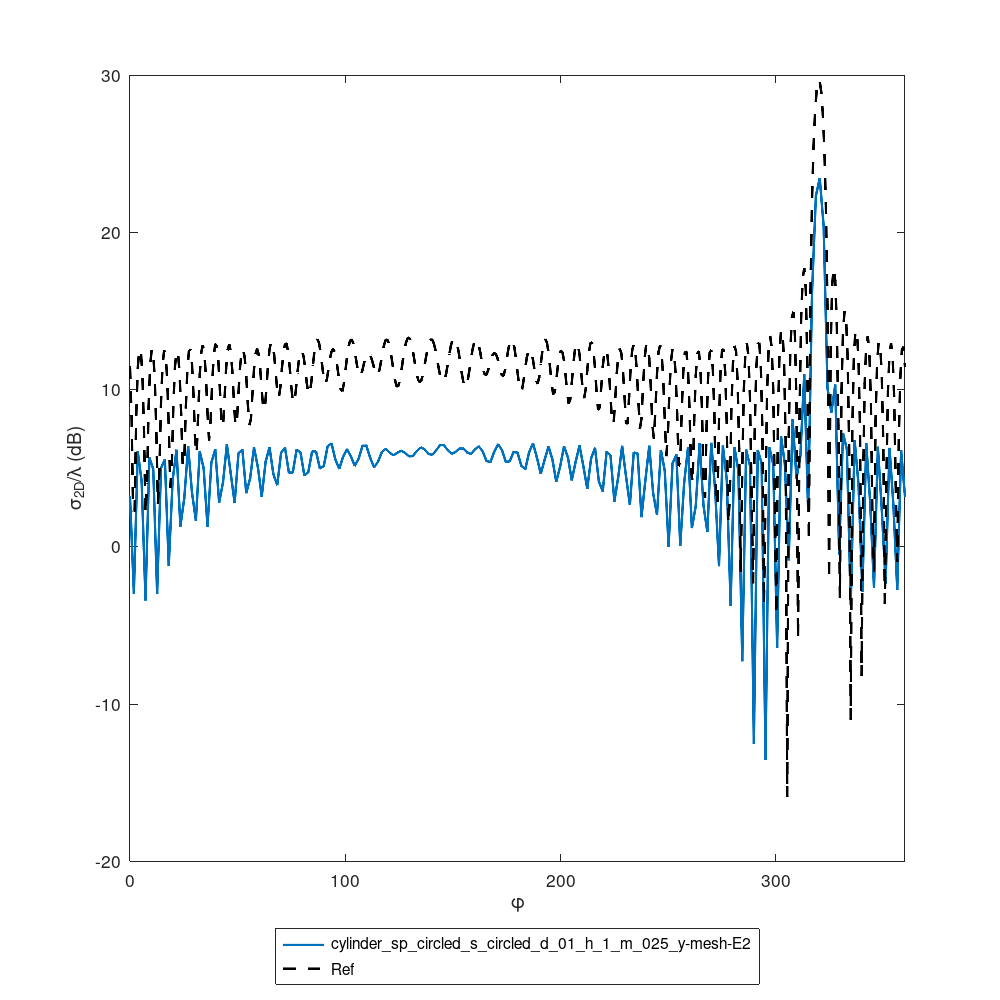
\includegraphics[width=\linewidth]{results/FF/cylD_01_H_1_M_025_Y/epr2_TE.png}

\column{0.23\textwidth}

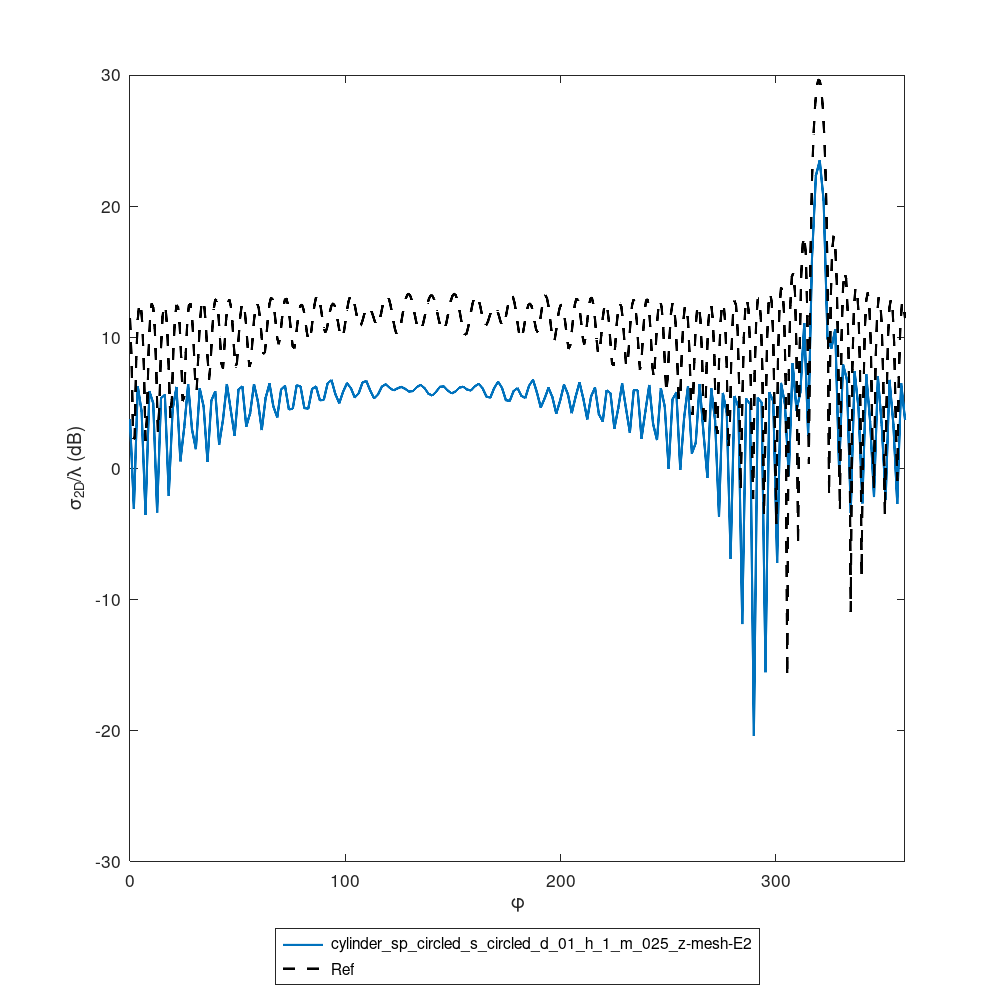
\includegraphics[width=\linewidth]{results/FF/cylD_01_H_1_M_025_Z/epr2_TE.png}

\column{0.23\textwidth}

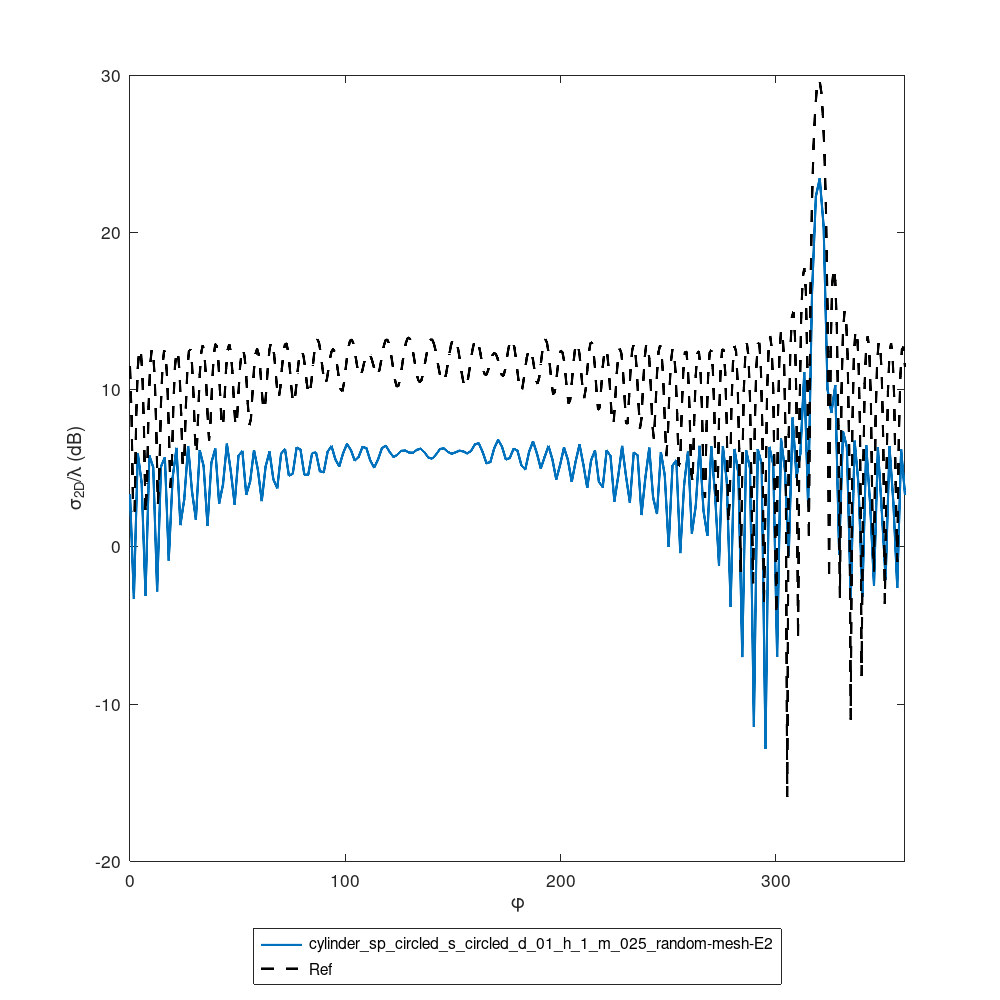
\includegraphics[width=\linewidth]{results/FF/cylD_01_H_1_M_025_RANDOM/epr2_TE.png}

\end{columns}

\vbs

Analytical curves and FEM curves agree (some discrepancies) except for a constant factor. 

Normalized bistatic-RCS:

\vbss

\begin{columns}
\column{0.23\textwidth}

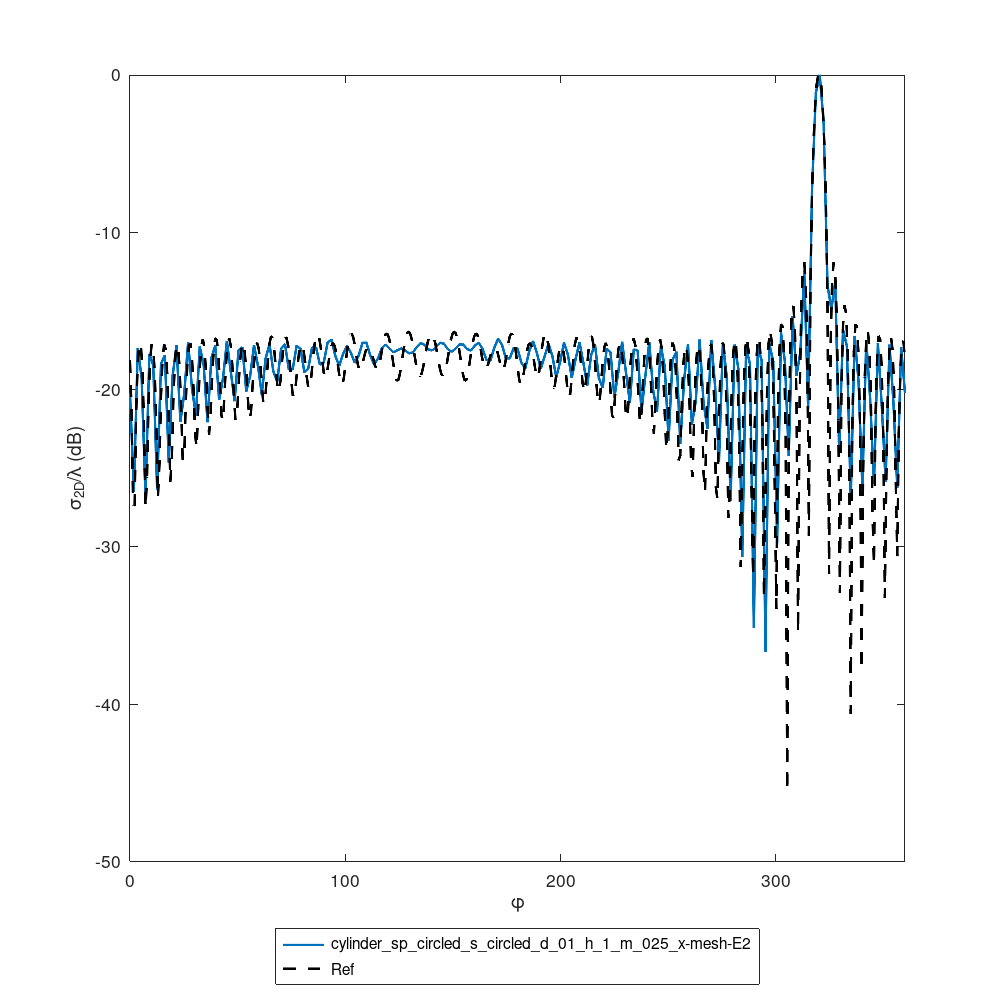
\includegraphics[width=\linewidth]{results/FF/cylD_01_H_1_M_025_X/epr2_TE_norm.png}

\column{0.23\textwidth}

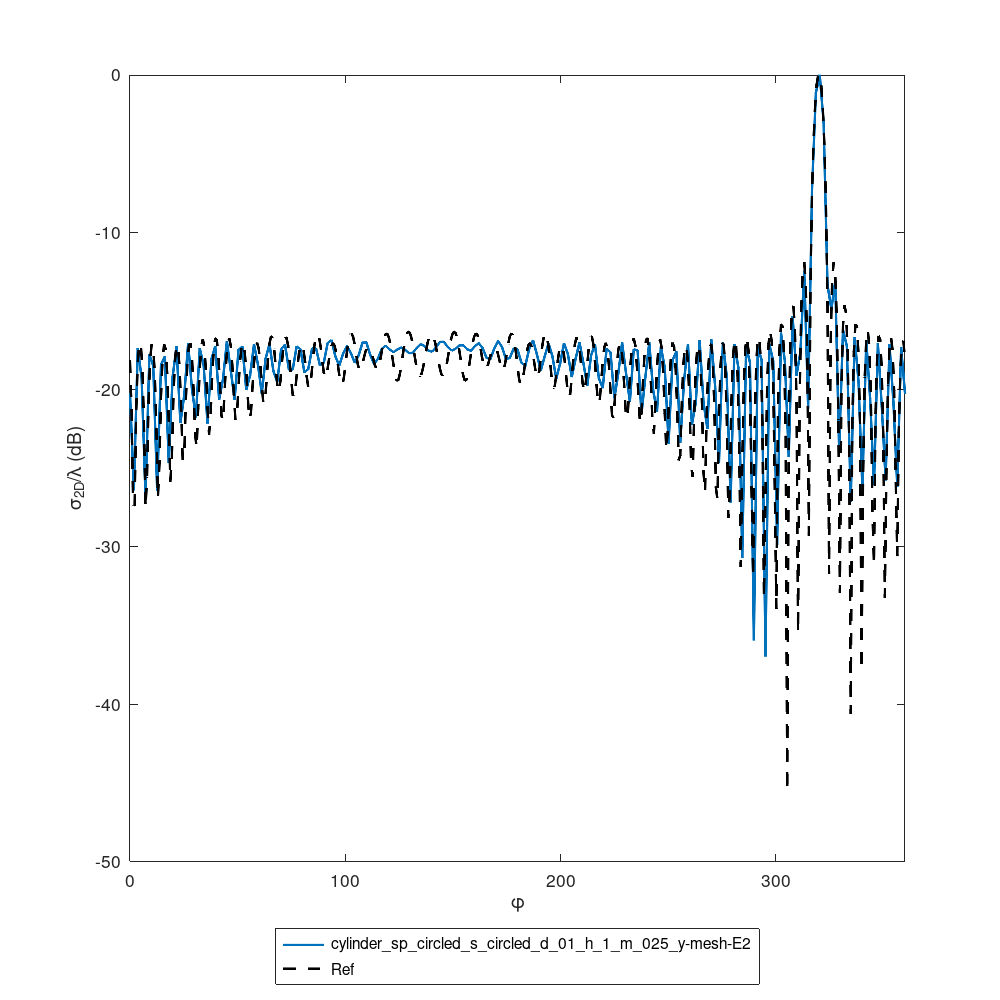
\includegraphics[width=\linewidth]{results/FF/cylD_01_H_1_M_025_Y/epr2_TE_norm.png}

\column{0.23\textwidth}

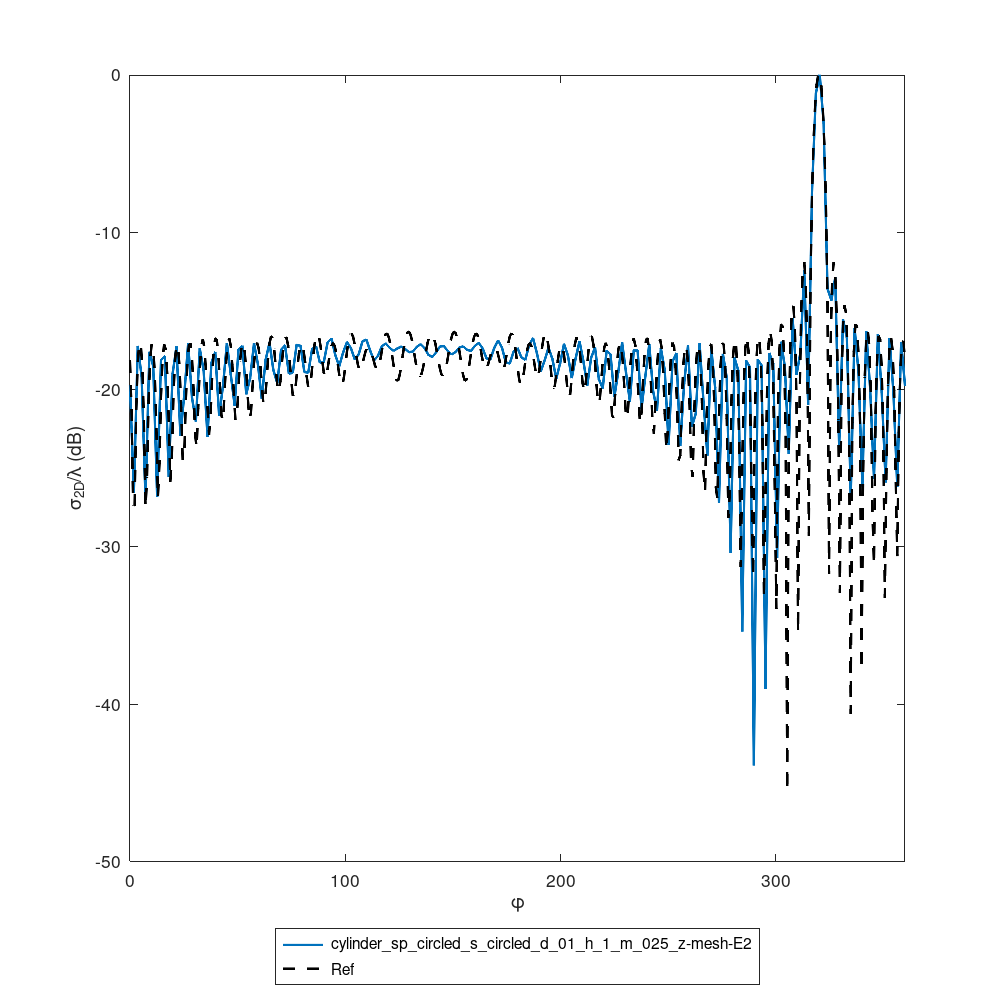
\includegraphics[width=\linewidth]{results/FF/cylD_01_H_1_M_025_Z/epr2_TE_norm.png}

\column{0.23\textwidth}

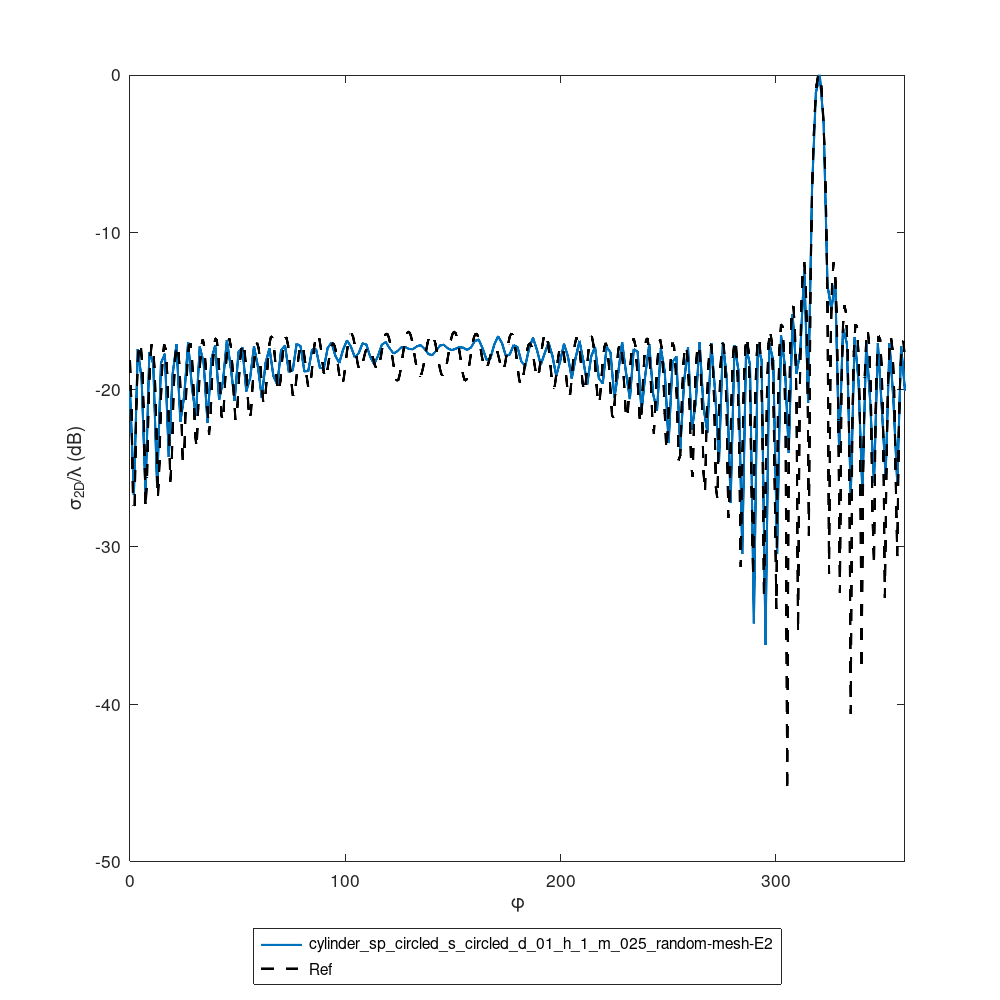
\includegraphics[width=\linewidth]{results/FF/cylD_01_H_1_M_025_RANDOM/epr2_TE_norm.png}

\end{columns}

\end{frame}

%%%%%%%%%%%%%%%%%%%%%%%%%%%%%%%%%%%%%%%%

\begin{frame}{TE polarization, $\varepsilon_r=2$, $f=150$\, MHz}

\begin{columns}
\column{0.23\textwidth}

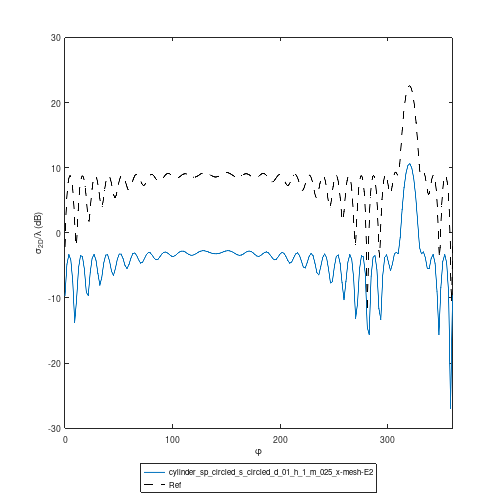
\includegraphics[width=\linewidth]{results/FF/cylD_01_H_1_M_025_X/epr2_TE_f150.png}

\column{0.23\textwidth}

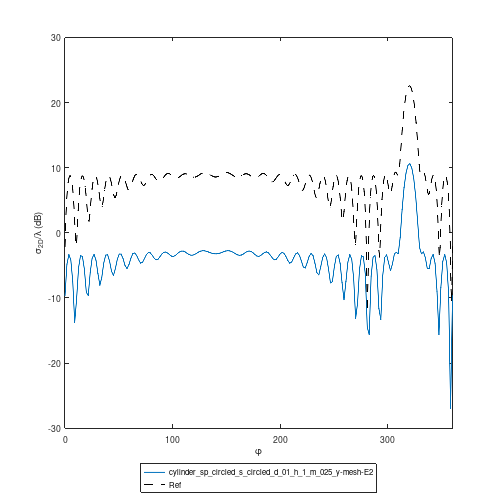
\includegraphics[width=\linewidth]{results/FF/cylD_01_H_1_M_025_Y/epr2_TE_f150.png}

\column{0.23\textwidth}

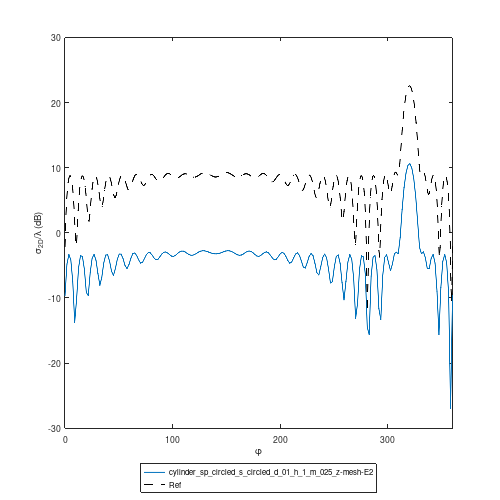
\includegraphics[width=\linewidth]{results/FF/cylD_01_H_1_M_025_Z/epr2_TE_f150.png}

\column{0.23\textwidth}

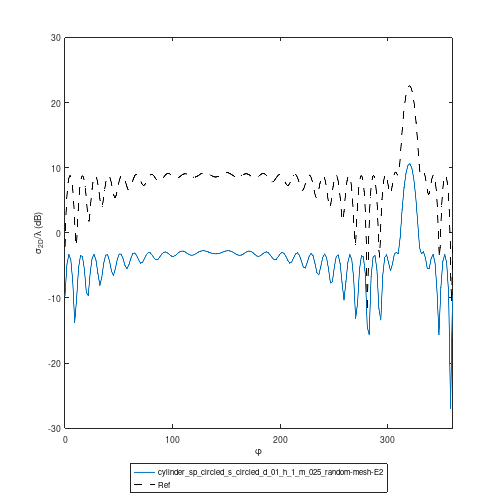
\includegraphics[width=\linewidth]{results/FF/cylD_01_H_1_M_025_RANDOM/epr2_TE_f150.png}

\end{columns}

\vbs

For a smaller problem (same mesh, double wavelength), almost full agree.

Normalized bistatic-RCS:

\vbss

\begin{columns}
\column{0.23\textwidth}

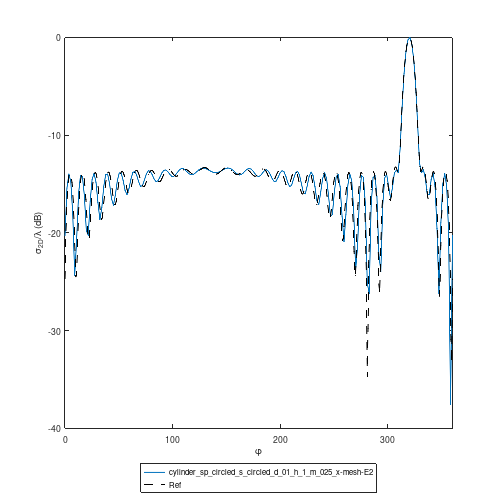
\includegraphics[width=\linewidth]{results/FF/cylD_01_H_1_M_025_X/epr2_TE_f150_norm.png}

\column{0.23\textwidth}

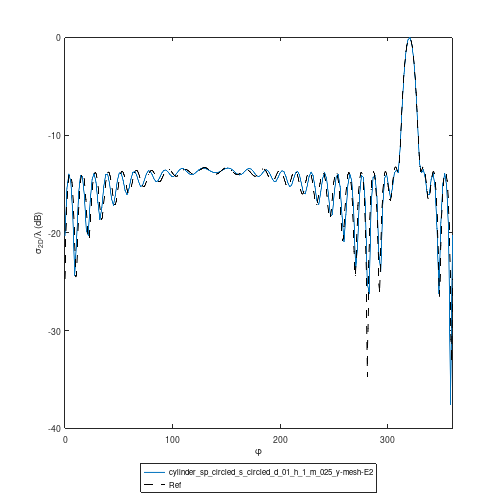
\includegraphics[width=\linewidth]{results/FF/cylD_01_H_1_M_025_Y/epr2_TE_f150_norm.png}

\column{0.23\textwidth}

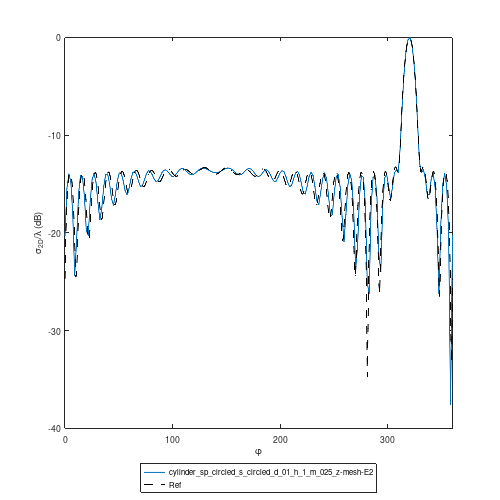
\includegraphics[width=\linewidth]{results/FF/cylD_01_H_1_M_025_Z/epr2_TE_f150_norm.png}

\column{0.23\textwidth}

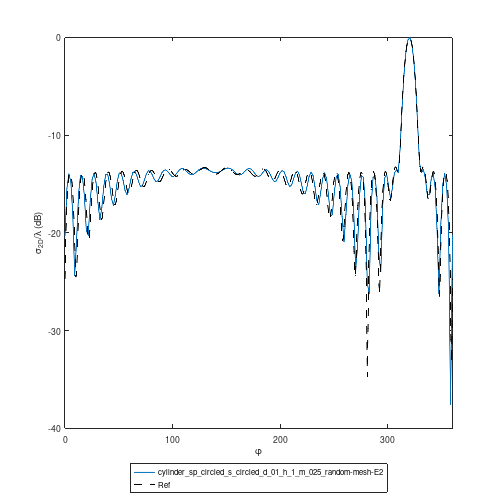
\includegraphics[width=\linewidth]{results/FF/cylD_01_H_1_M_025_RANDOM/epr2_TE_f150_norm.png}

\end{columns}

\end{frame}

%%%%%%%%%%%%%%%%%%%%%%%%%%%%%%%%%%%%%%%%

\begin{frame}{Effect of IIEE iterative method in Far Field}{TM polarization, $\varepsilon_r=1$, (reference case)}

Results for the following residual errors:
\begin{itemize}
\item \texttt{M1}: $10^{-1}$ (blue)
\item \texttt{M2}: $10^{-2}$ (red)
\item \texttt{M3}: $10^{-3}$ (orange)
\end{itemize}


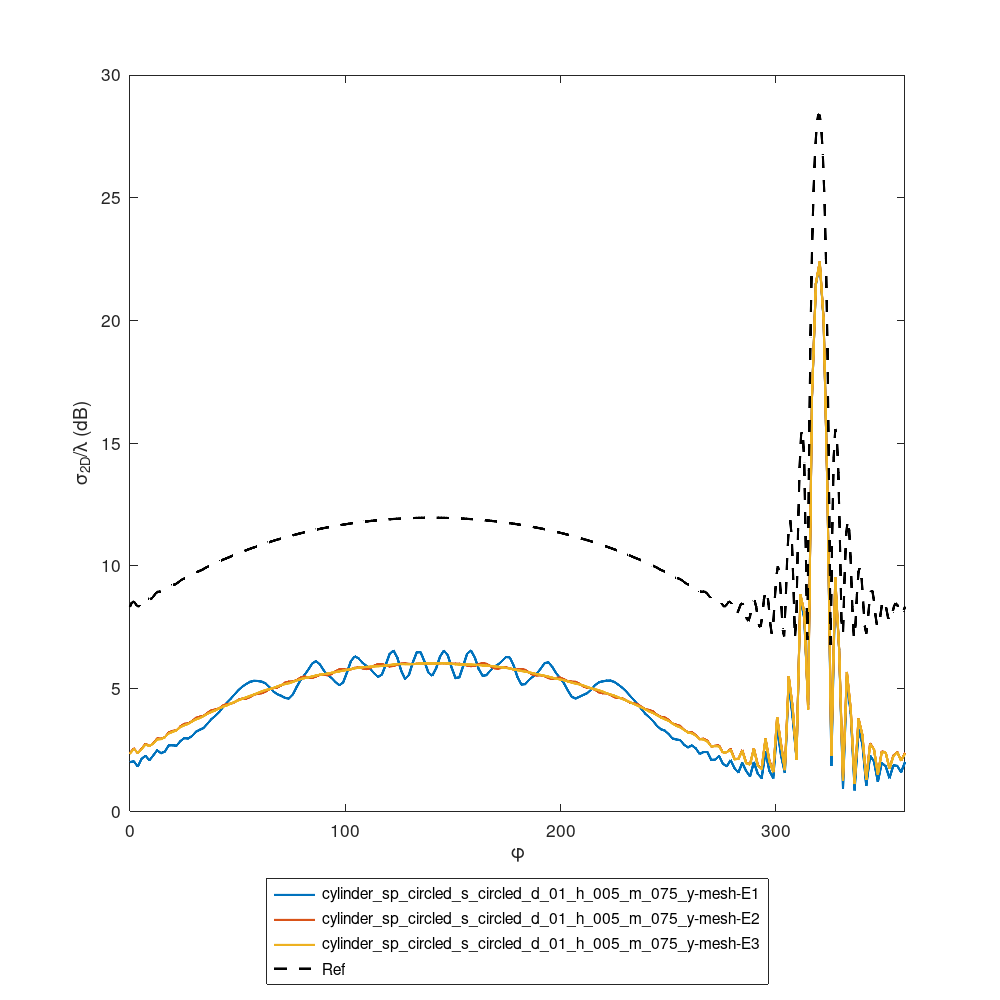
\includegraphics[width=0.45\linewidth]{results/FF/cylD_01_H_005_M_075_Y/iiee075.png}
\hfill
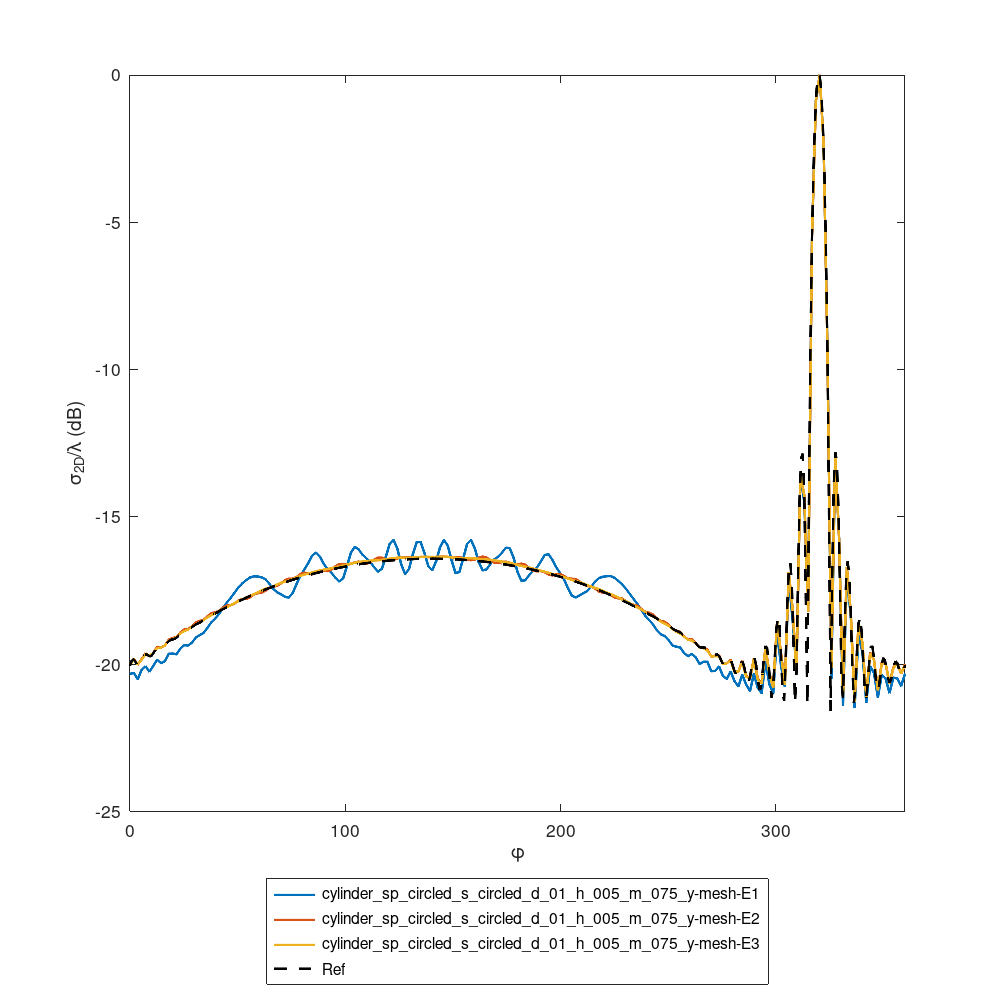
\includegraphics[width=0.45\linewidth]{results/FF/cylD_01_H_005_M_075_Y/iiee075_norm.png}


Note: Orange and red lines overlap. 

\end{frame}
